\documentclass[twoside,12pt]{mythesis} %this is the mythesis.cls file
% twoside,openright,versioninfo

% Consider:
% \newcommand{\ie}{i.\,e.}
% \newcommand{\Ie}{I.\,e.}
% \newcommand{\eg}{e.\,g.}
% \newcommand{\Eg}{E.\,g.}
\usepackage{graphicx}
\usepackage{amsmath}
\usepackage{booktabs}
\usepackage{capt-of}
\usepackage{enumerate}
\usepackage{array} %Use this to centre table columns that are a pre-defined width



%You might need to load other packages here...
\setcounter{tocdepth}{4}
\setcounter{secnumdepth}{4} %number of subsections that are allowed
 
	%I added these to try and get subsubsections to work but I could only get the numbering into the table of contents and not in the text
	
	

%% Symbols
% unresolved:
\newcommand{\ud}{\mathrm{d}}
\newcommand{\drel}{\ensuremath{r_{\mathrm{rel}}}}
\newcommand{\nmax}{\ensuremath{n_\mathrm{max}}}

%Information for the title page
%Some of this is hard coded in mythesis.cls but you can over write if you need to
\title{Morphological diversity in tenrecs (Afrosoricida, Tenrecidae)}

% NC: Not sure on the title. Really you're looking at morphological diversity in tenrecs, not in their evolution as such. Maybe just Morphological diversity in tenrecs? Really the title should be the answer to the overall question you're asking, or the question itself
	%SF: Alternative: Morphological diversity in tenrecs compared to their closest relatives?

%
\author{Sive Finlay}
%
\month{\textsc{January}} \year{2015}
\previousdegrees{B.A. (Mod) Zoology, Trinity College Dublin 2012}
\degreetitle{Masters by Research}
\institution{Trinity College Dublin}
\school{School of Natural Sciences}
\department{Zoology}

%End of preamble.
%--------------------------------------
\begin{document}

\maketitle %puts in your title

\chapter*{Abstract}
\chaptermark{abstract}
\addcontentsline{toc}{chapter}{Abstract}

Here is the abstract of my thesis.

%

%%% Local Variables:
%%% TeX-master: "thesis"
%%% TeX-PDF-mode: t
%%% End:
 %inputs abstract.tex
\allcontents %tells it to make a table of contents with figure and table lists too
% There is currently a problem with spacing somewhere so that Table of
% Contents, List of Tables, and List of Figures have the wrong amount
% of space.  Others are OK though...
\chapter*{Acknowledgements}
\addcontentsline{toc}{chapter}{Acknowledgements}

I would like to acknowledge Dr Rich FitzJohn for letting me use his thesis template!

%%% Local Variables:
%%% TeX-master: "thesis.tex"
%%% TeX-PDF-mode: t
%%% End:
 %inputs acknowledgements.tex
\cleardoublepage
\mainbody

\chapter{Introduction}
\label{chap:introduction}



\noindent
Thesis introduction
Patterns of diversity, morphological differences, geometric morphometrics overview

\section{Tenrecs are cool}




\section{Diversity within tenrecs}

Adaptive radiations and morphological disparity

\section{Convergence}
Similarities among tenrecs and other species



\section{Structure \& contents of this thesis}
Brief introduction of each section
%
%In \chapref{labstudy}, I do some lab work.
%
%In \chapref{velociraptor}, I train a velociraptor to ride a hoverboard.
%
%Finally, in \chapref{conclusions}, I close with a discussion of the
%limitations of the methods used in the thesis, and suggest some future
%directions.

 

\chapter{Methods}
\label{chap:methods}

\section{Introduction}

	I compiled a morphological data set of both photographs and linear measurements from 366 specimens representing 101 species of small mammals. %(total number of skulls and species in Access Data base)
	I collected morphological data from skulls, limbs and skins and here I included the details of how I compiled each of these data sets. I have only analysed the skulls' data in detail so the information I collected on limbs and skins represent significant resources for future work %put in reference to the future work section in the last chapter 
	
	I have divided my description of how the data were collected and analysed into four sections:
	
	\begin{enumerate}[i]
	
	\item Data collection (section \ref{sect:datacollection}): \\
	Summary of the species measured, information recorded from the museums' labels, linear measurements and photographic set up.
	
	\item Geometric morphometric analyses (section \ref{sect:morphometrics}):\\
	Landmark and semilandmark placements on different views of skulls and mandibles.
	
	\item Error checking (section \ref{sect:errors}): \\
	How I dealt with errors in taxonomic and specimen identification, possible variation associated with sex and age class, accuracy and repeatability of linear measurements and morphometric errors associated with photographing specimens and the placement of landmarks.
	
	
	\item Quantifying disparity and convergence (section \ref{sect:data_analysis}):\\
	Statistical approaches to measuring patterns of cranial diversity in small mammals.
	
	\end{enumerate} 


%####################################################
\section{Data collection}
\label{sect:datacollection}
%##################################################


\subsection{\normalfont{Species measured and taxonomy}}

	Between January and September 2013, I spent a total of 9 weeks working in the collections of five museums: the Natural History Museum London (NHML), the Smithsonian Institute Natural History Museum (SI), the American Museum of Natural History (AMNH), Harvard’s Museum of Comparative Zoology (MCZ) and the Field Museum of Natural History (FMNH), Chicago. I compiled measured and photographed 366 skulls, 248 post-cranial skeletons and 277 skins from 101 species belonging to four mammalian orders; Afrosoricida, Erinaceomorpha, Soricomorpha and Notoryctemorphia. 
	These belonged to seven families of mammals; tenrecs (Tenrecidae), golden moles (Chrysochloridae), hedgehogs and gymnures(Erinaceidae), shrews (Soricidae), solenodons (Solenodontidae), moles and desmans(Talpidae) and marsupial moles (Notoryctidae).
	%Put in a new summary table of all of the different measurements
	I measured all of the tenrecs and their sister taxa the golden moles that were available in the collections %Put in the numbers of how many species this includes.(total of 43 species in the skdors data)
	For my comparative species of non-Afrosoricida species, I chose a random sample of 52 taxa %non tenrec or golden mole species in the skdors data) 
	which have been previously identified as convergent with tenrecs \citep[e.g.][]{Gould1966, Symonds2005, Poux2008, Olson2013}.Following the taxonomy in Wilson and Reeder's Mammal Species of the World (MSW) \citeyearpar{Wilson2005}, I used phylogenies for each order to select species at random which represented the main sub-branches and morphological diveristy of each order. For example, within the Soricomorpha, I included both species of \textit{Solenodon} but only 3 %number of Crocidura species in Access data base
	(out of a total of xx) species of \textit{Crocidura} as the former genus represents a separate subgroup to the rest of the order. 

	I used the taxonomy of Wilson and Reeder \citeyearpar{Wilson2005} supplemented with more recent sources \citep{IUCN2012, Olson2013} to identify our specimens. Table \ref{tab:species.measured} outlines the number of species I measured from each family and how this sample relates to the overall number of species in that group as recorded by both MSW and the IUCN.

%####################################################
%Species.measured table: I need to fill in the correct numbers

\begin{table}[h]
	\caption[Summary of species measured] 
	{The number of species I measured in each family compared to the total number of species in that family according to two sources; \citep{Wilson2005} and \citep{IUCN2012}}
	%Species.measured table
%To get the number measured for each Family, I counted the number of unique species in my Tb_Taxonomy Access table for that family
%So it's the number of species measured overall but that doesn't necessarily mean that I have the same number in every data set
%I didn't count the _sp. specimens as separate species

%I took out the reference to the IUCN because it seems to only list species that are threatened/endangered rather than a full list of all species in a family

\begin{tabular}{p{3.4cm}p{3cm}p{2cm}p{2cm}p{2cm}}

\hline
\textbf{Order} & \textbf{Family} & \textbf{Measured species} & \textbf{Total species} & \textbf{Coverage} \\
\hline
%----------------------------------------------------
Afrosoricida & Tenrecidae & 31 & 34 & 91 \% \\
%-------------------------------------------------
Afrosoricida & Chrysochloridae & 12 & 21 & 57 \% \\
%----------------------------------------------------
Erinaceomorpha & Erinaceidae & 16 & 24 & 67 \% \\
%----------------------------------------------------
Soricomorpha & Soricidae & 22 & 376 & 5.8 \% \\
%----------------------------------------------------
Soricomorpha & Solenodontidae & 2 & 4 & 50 \% \\
%----------------------------------------------------
Soricomorpha & Talpidae & 15 & 39 & 38 \% \\
%----------------------------------------------------
Notoryctemorphia & Notoryctidae & 1 & 2 & 50 \% \\
%-----------------------------------------------
\hline

\end{tabular}

%*There are now 34 recognised tenrec species \citep{Olson2013}
	\label{tab:species.measured}
\end{table}

%####################################################
%-----------------------------------	
%I took out this section because it's just saying that there are extra tenrec species but I'm not measuring them

	%Although MSW is a comprehensive mammalian taxonomic reference, it does not include some known species. For example, Wilson and Reader \citeyearpar{Wilson2005} record 30 species of tenrec but more recent studies indicate that there are now 34 recognised species of tenrec \citep{Olson2013}. The additional species belong to the shrew tenrec (\textit{Microgale}) genus and represent either recognition of cryptic species boundaries \citep{Olson2004} or discovery of new species \citep{Goodman2006, Olson2009}. Only one of these four recent additions to the \textit{Microgale} genus, \textit{M. jobihely}, was present in museum collections and therefore I could not include the three other newly recognised species in my analyses.


%------------------------------------------------------


\subsection{\normalfont{Museums' label data}}

	I recorded all the data on the specimen labels including any handwritten or printed notes which had been added by other users of the collection. The label data included the museum specimen ID number, genus, species, sex, collector’s name, the date and location of where the specimen was collected. Some of the labels attached to skins had additional information such as the body, tail, hind foot and ear lengths as well as the body mass of the live individual. 
	The level of detail recorded on the labels varied considerably (figure \ref{fig:museum.labels}). For example recently collected specimens were more likely to have detailed information about the collection location, and some specimens did not have even basic information such as the sex recorded. 

%Museum label pictures

\begin{figure}[h] 
  \centering
  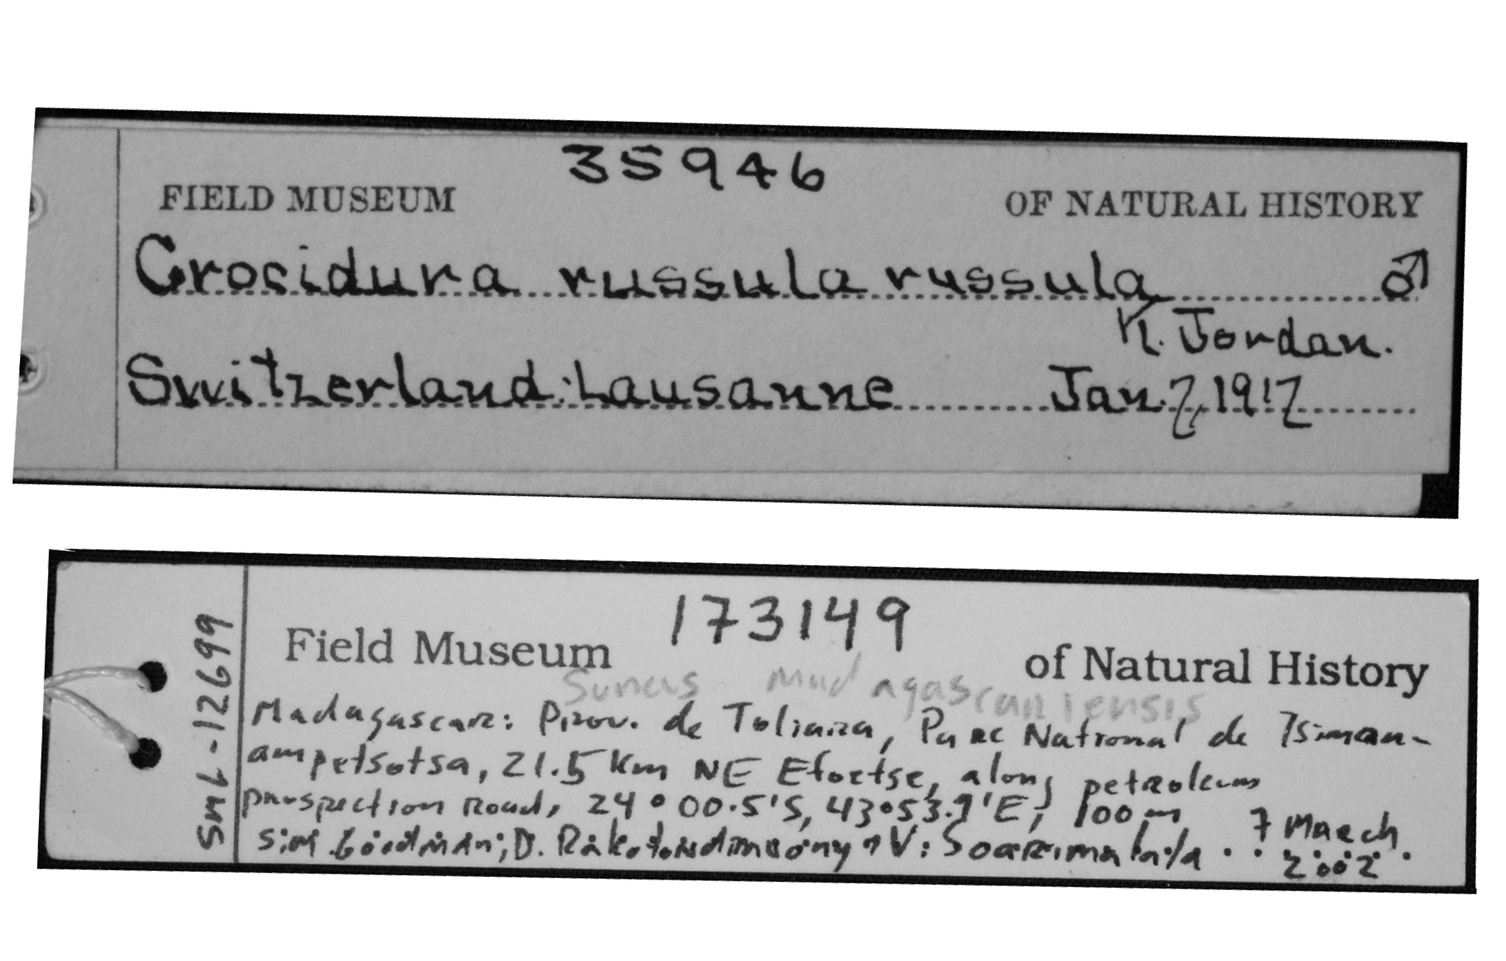
\includegraphics[width = 15cm, height = 15cm, keepaspectratio=true]{Methods/figures/labels.png}
    \caption[Examples of museum labels]
    {Examples of the variation in the detail of information which is available from museum labels}%this is under the figure
  \label{fig:museum.labels}
\end{figure}
  
%------------------------------------------------
\subsection{\normalfont{Linear measurements}} 
\label{sect:measurements} %Label the section so I can refer to it in the error checking later on

	Using a 15mm digital calipers (Mitutoyo Absolute digimatic calipers), I took 20 measurements of the skulls and mandibles (table \ref{tab:sk.measurements}) and 19 measurements of the limbs (table \ref{tab:limb.measurements}). My choice of which measurements to include was based on three main criteria; 1) their relevance to biological and ecological traits such as diet specialisation and locomotory adaptation, 2) their usefulness for assessing the overall shape and size of the specimen and 3) the ease with which they could be repeated both within and among specimens from different species. 
	Figures x-x depict the linear measurements of skulls and figures xx show the limb measurements. %I haven't made these pictures or filled in the tables yet

	I took each linear measurement three times, cycling through all 20 skull or 19 limb measurements then repeating the cycle to avoid measuring the same variable twice in a row. Small measurements (<2 mm) are particularly prone to high error rates \citep{Cardini2008}. Therefore, I took five separate replicates of some of the variables which were most prone to errors (marked with PUT IN SYMBOL in tables \ref{tab:sk.measurements} and \ref{tab:limb.measurements}). These included four of the skull measurements (PWa, IncisorH, IFD and IFcanal) and five of the limb measurements (FemD, TibD, HumD, UlnD, RadD). 
	Five replicates should give a more reliable median value because even if there are one or two outlying measurements there should be at least three replicates which are in close agreement \citep{Cooper2009}.

%******************************
%I need to create the diagrams and fill in these tables

% Skull and mandible measurements

\begin{table}[h]
	\caption[Description of the skull and mandible measurements]
			{Skull and mandible measurements}% add to this caption
	%Skull measurements

\begin{tabular}{lp{3.5cm}p{9.75cm}}
\hline
\textbf{Abbreviation} & \textbf{Measurement} & \textbf{Description}\\
\hline
CB & Condylobasal length & Total skull length from the front of the premaxillary  bones to the rear of the occipital condyles, measured from below \\
%-------------------------------------------
PL & Palate length & Maximum length of the palate from the anterior of the pre-maxilla to the posterior of the hard palate\\
%----------------------------------------------
TR & Tooth row length & From the front of the alveolus of the first incisor to the rear of the alveolus of the last molar on the same side\\
%----------------------------------------------
PWa* & Palate width anterior & Width across the palate measured between the posterior, outer-most points of the alveoli of the first pair of teeth\\
%I had to modify this measurement slightly for some species: when there was a row of anterior incisors which stretch across the front of the palate (e.g. Euroscaptor klossi SI_261090) then I measured PWa as the width across from back of the row of the incisors on either side (i.e. just in front of the canines) 
%----------------------------------------
maxPW & Maximum palate width & Measured at the widest point of the palate\\
%--------------------------------------------
IncisorH* & Incisor height & Maximum height of the first incisor on the right\\
%----------------------------------------
ZW & Zygomatic width & Maximum width between the zygomatic arches (measured within the arches from below the skull)\\
%---------------------------------------
MX & Maxilla width & Width between the maxillary bones, measured from above the skull. Species with zygomatic arches; width from the innermost connection between the anterior of the arch and the skull. No arches; width between the anterior skull constrictions.\\ 
%---------------------------------------
SQ & Squamosal width & Width between the squamosal bones, measured from above the skull. Species with zygomatic arches; width from the innermost connection between the posterior of the arch and the skull. No arches; width between the posterior skull constrictions \\
%-------------------------
OL & Orbit length & Longitudinal length of the orbit opening measured along the edge of the skull from the maxilla to the squamosal. \\
%------------------------------
IFD* & Interorbital foramen width & The maximum (vertical) diameter of the right interorbital foramen\\
%-----------------------------------------------
IFW & Interorbital foramen width & Maximum width across the skull between the two interorbital foramina, measured from above\\
%-------------------------------
IFcanal* & Interorbital foramen canal & Length of the right IF canal measured between the anterior and posterior openings from above\\
%---------------------------------
BW & Braincase width & Width across the braincase at the widest point of the skull\\
%---------------------------------
SkH & Skull height & Perpendicular height from the highest point on the braincase to the base of the skull\\



\hline
\end{tabular}
	\label{tab:sk.measurements}
\end{table}


% Limb measurements
\begin{table}[h]
	\caption[Description of the limb measurements]
		{Limb measurements} % add to this caption
	%Limb measurements


\begin{tabular}{lp{3.5cm}p{9.75cm}}
\hline
\textbf{Abbreviation} & \textbf{Measurement} & \textbf{Description}\\
\hline
Inn & Innominate length & Maximum longitudinal length of the pelvic bone measured in a straight line from the anterior tip to the posterior curve \\ 
%-----------------------------------
Obt & Obturator foramen & Maximum diameter of the opening in the pelvic bone \\
%-----------------------------------
FemL & Femur length & Length of the bone excluding the femoral head (i.e. length of the bone without the joint area)  \\
%-----------------------------------
FemD* & Femur diameter & Minimum width across the shaft of the bone \\
%-----------------------------------
TibL & Tibia length & Maximum longitudinal length of the tibia  \\
%-----------------------------------
TibU & Tibia unfused length & Length of the tibula which is not fused with the fibula \\
%-----------------------------------
TibD* & Tibia diameter & Minimum diameter across the shaft of the tibia bone \\
%-----------------------------------
Foot & Foot length & Maximum length of the entire foot (heel to longest toe) \\
%-----------------------------------
Toe & Toe length & Length of the longest toe bone (just the phalange bone up to the metatarsal joint) \\
%-----------------------------------
ScapL & Scapula length & Perpendicular length of the scapula from the curved end to the anterior point  \\
%-----------------------------------
ScapW & Scapula width & Maximum perpendicular width across the bone \\
%--------------------------------
HumL & Humerus length & Maximum length of the bone. In golden moles (L-shaped humerus): diagonal distance between the two ends of the bone  \\
%-------------------------------
HumLvert & Humerus length vertical & Only for golden moles with L-shaped humerus: length of the vertical (longer) side of the bone \\
%-------------------------------
HumLhori & Humerus length horizontal & Only for golden moles with L-shaped humerus: length of the horizontal (shorter) side of the bone \\
%-----------------------------------
HumD* & Humerus diameter & Minimum diameter across the shaft of the humerus \\
%-----------------------------------
UlnL & Ulna length & Length of the bone from the posterior tip to the wrist joint \\
%-----------------------------------
RadL & Radius length & Length of the bone from the posterior tip to the wrist \\
%--------------------------------
UlnD* & Ulna diameter & Minimum diameter across the ulna \\
%-------------------------------
RadD* & Radius diameter & Minimum diameter across the radius \\
%----------------------------
Hand & Hand length & Maximum length of the entire hand (wrist to longest finger) \\
%------------------------
Finger & Finger length & Length of the longest finger bone (to the metatarsal joint) \\
%---------------------
\hline

\end{tabular}
	\label{tab:limb.measurements}
\end{table}


%****************************
%####################################################
\subsection{\normalfont{Photographing set up}}
%I tried to have this as a subsubsection under a subsection of Landmark morphometrics but the subsubsection numbering only appears in the table of contents, not here in the main body of the text

	In order to get 2D landmarks for my specimens, I first had to photograph them. I used photographic copy stands consisting of a camera attachment with an adjustable height bar, a flat stage on which to place the specimen and an adjustable light source to either side of the stage. I used the copy stands that were available at each museum which differed in how the camera height was adjusted and in the light sources available.
	To take the light variability into account, on each day I took a picture of a white sheet of paper and used the custom white balance function on the camera to set the image as the baseline “white” measurement for those particular light conditions.
	
	I photographed the specimens with a Canon EOS 650D camera fitted with either an EF 100mm f/2.8 Macro USM lens (skulls and limbs) or EFS 18-55mm lens (skins). I used a remote control (h\"ahnel Combi TF) to take the photos to avoid shaking the camera and distorting the images. I photographed the specimens on a black material background. I placed the light source from the top left-hand corner of the picture and positioned a piece of white card on the bottom right side of the specimen which reflected the light back onto the specimen and minimised any shadows (figure \ref{fig:camera} below).

	I made small bean bags (12 x 5cm) from the same black material as the background and filled them with plastic beads. I used these bags as necessary to hold the specimens in position while being photographed. For example, when taking pictures of the lateral view of skulls, I placed one bean bag under the nose of the skull and another bag lying along the top (cranial) side of the skull to ensure that the side I was photographing lay in a flat plane relative to the camera and did not tilt in any direction. 
	I used the grid-line function on the live-view display screen of the camera to position the specimens in the centre of each image. 

%----------------------------------------------
%Camera picture
\begin{figure}[h] 
  \centering
  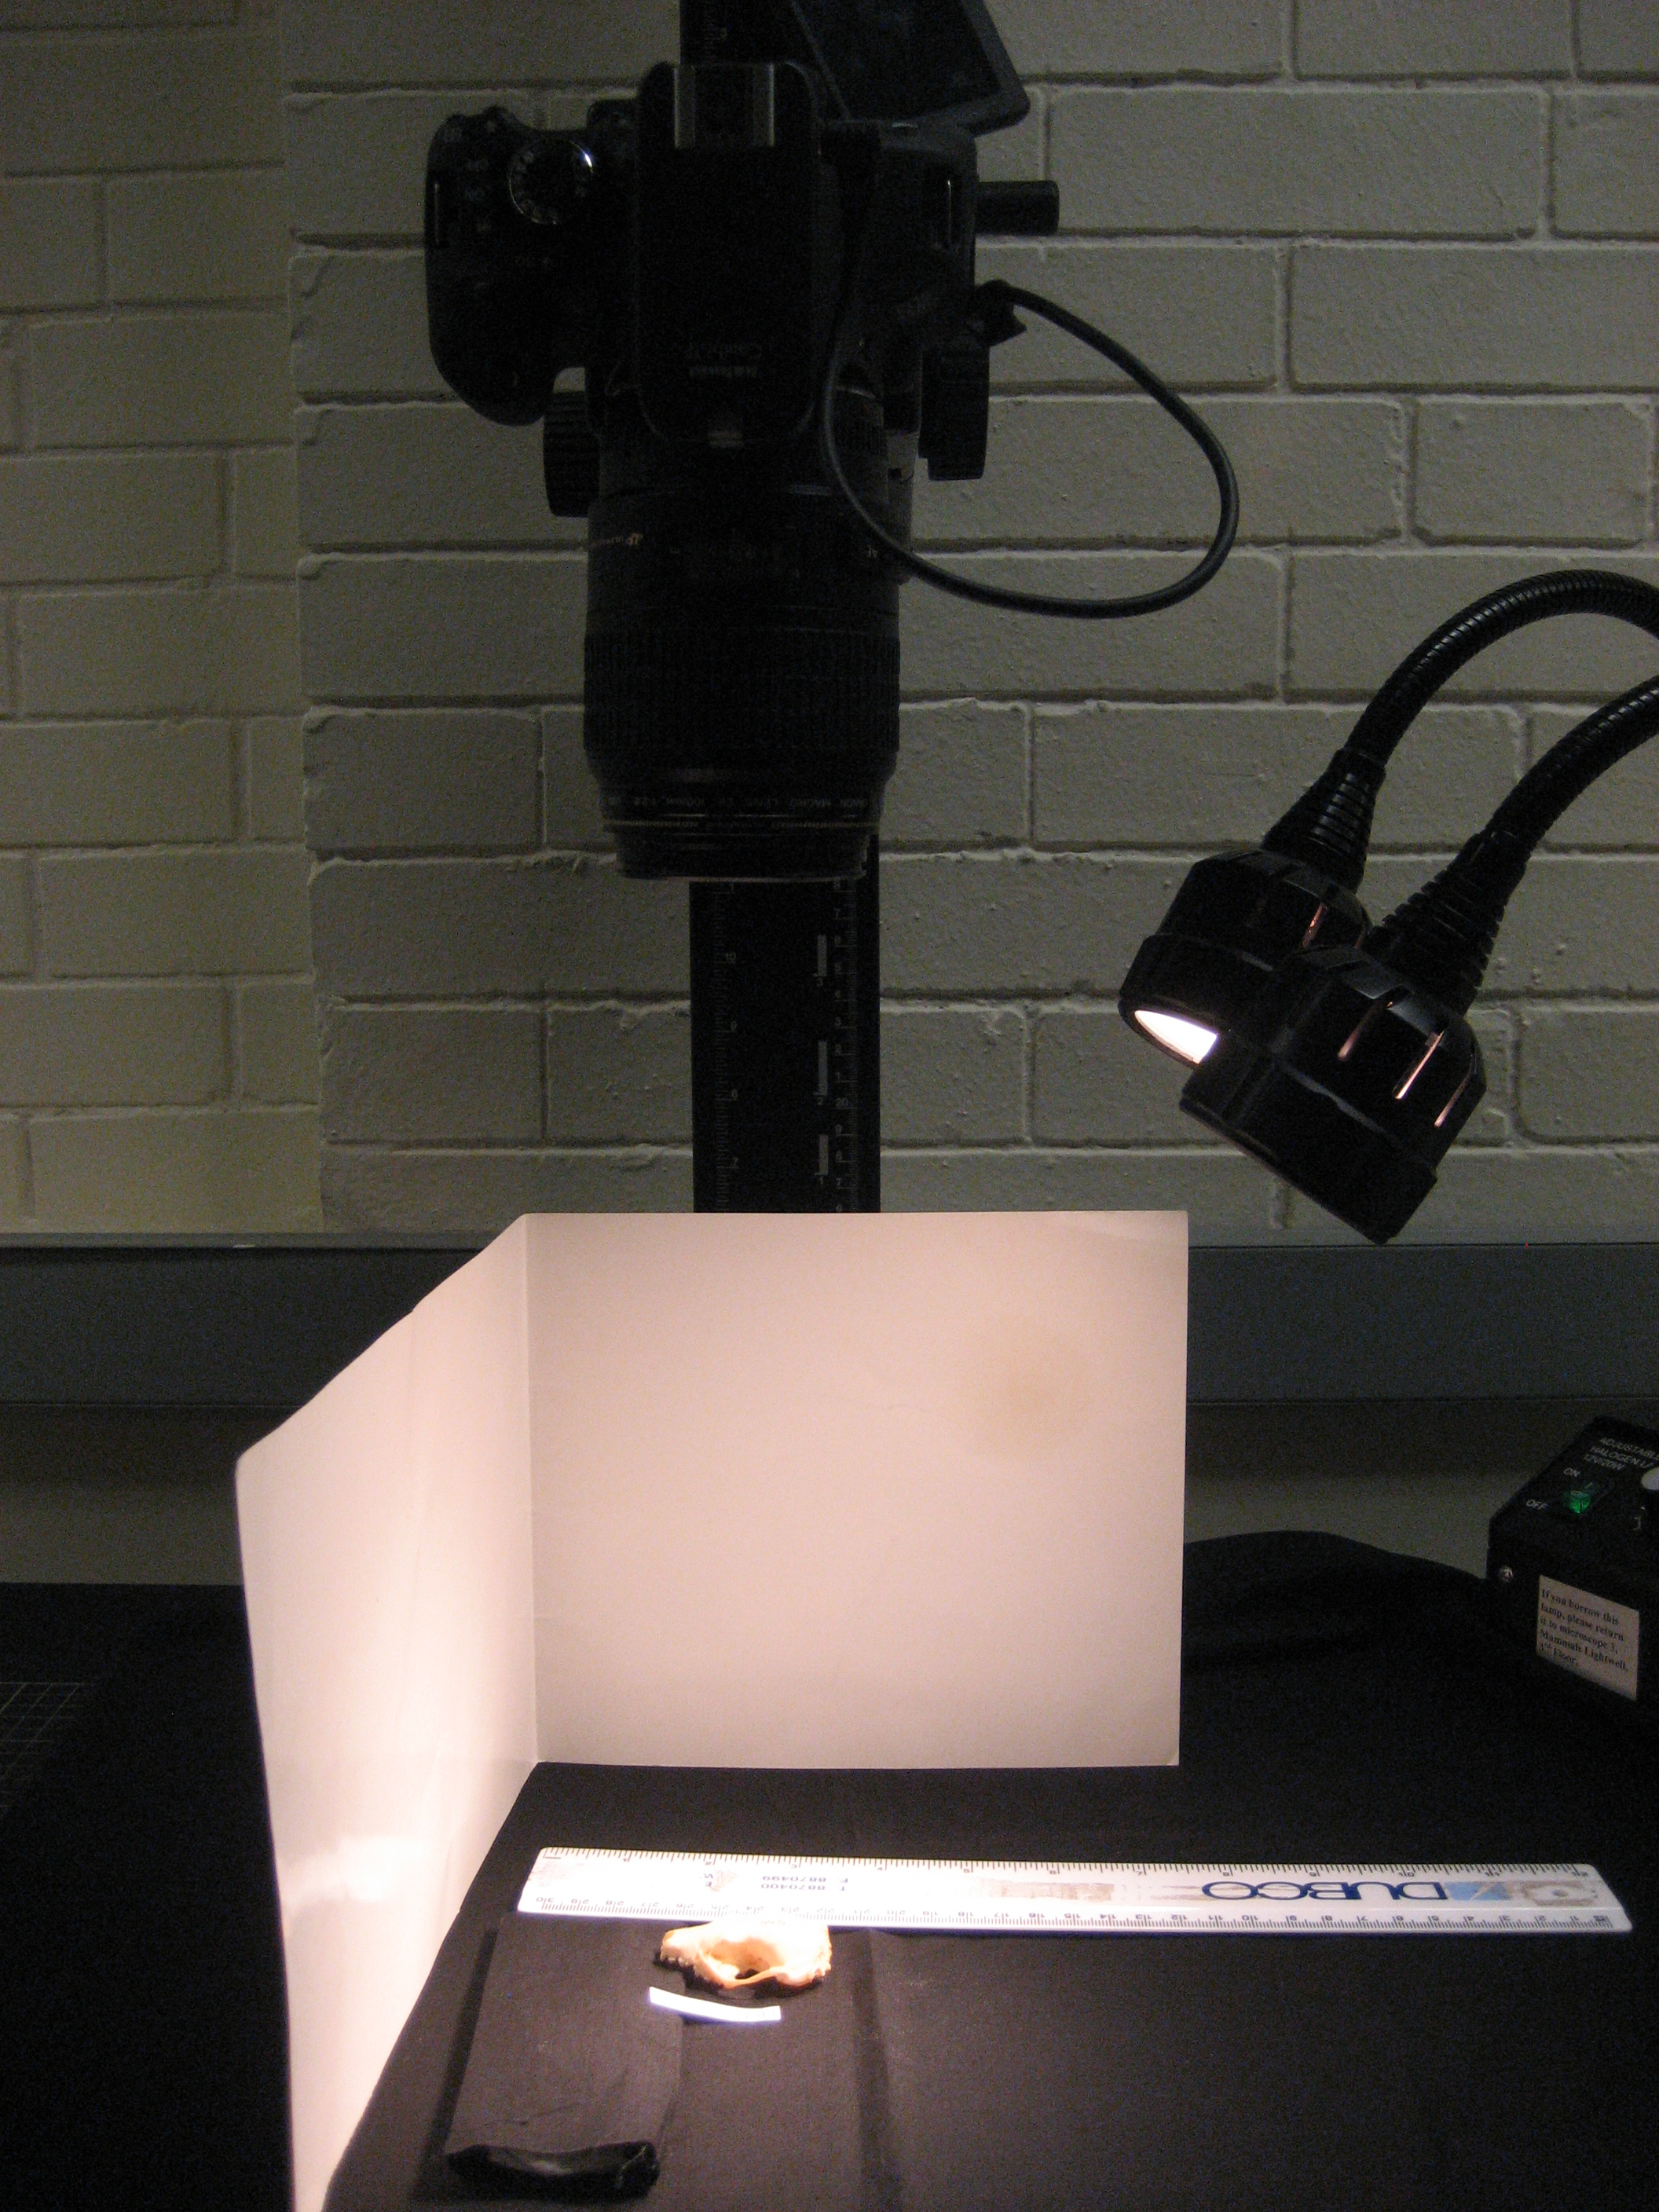
\includegraphics[width=12cm, height=12cm, keepaspectratio=true]{Methods/figures/camera.jpg}
    \caption[Photographic set up]%this is what appears in table of contents
    {Photographic set up for taking images of my skulls. The camera (above centre) is fitted to a copy stand, the light source is directed from the top-left corner of the image and the white card reflects the light back onto the skull. }%this is under the figure
  \label{fig:camera}
  \end{figure}
%-------------------------------------------------

\subsection{\normalfont{Photographing specimens}}
	I photographed the skulls in three views; dorsal (top of the cranium), ventral (underside of the skull with the palate roof facing uppermost) and lateral (right side of the skull). I also photographed the outer (buccal) side of the right mandible. When the right side of either the skull or mandibles were damaged or incomplete, I photographed the left sides and later reflected the images so that they could be compared to pictures of the right sides \citep[e.g.][]{Barrow2008}.

	Initially, I tried to take pictures of the limbs in similar orientations to the skulls (dorsal, ventral and lateral). However, there was considerable variation in how the limbs were preserved. For example, some limbs were still articulated while others had fragmented bones. It therefore proved impossible to place the limb bones in consistent orientations that would be comparable across species. Similarly, the small size of some limbs, combined with the frequently incomplete nature of postcranial museum collections, made landmark-based morphometric analyses of any limb pictures impractical. Therefore, I photographed the fore- and hind-limb bones in outer (the side facing away from the rest of the body) and inner (the side facing in towards the centre of the body) views for reference purposes only.

	As I was limited by the maximum camera height available on the copy stands, most skins were too large to be photographed with the 100mm macro lens. Therefore, I used an EFS 18-55mm lens to take pictures of the skins. I photographed skins in the same three orientations as the skulls; dorsal (the upper surface of the animal), ventral (the belly side of the skin) and lateral (right flank of the animal with the skin held in position using bean bags). The dorsal and ventral views give very approximate estimates of the overall body shape of the animal. The lateral views are less biologically relevant since the taxidermic process is unlikely to produce specimens which represent the true body height of the animal.

\subsection{\normalfont{Saving and processing images}}
	Photographs were captured and saved in a raw file format. Before using the pictures for morphometric analyses, I converted the raw files to binary (grey scale) images and re-saved them as TIFF files. The black and white pictures were more useful for later analyses since I was not interested in including any colour comparisons and it is easier to see some biological features in binary images. TIFF files were the most appropriate to use for my morphometric analyses as they are uncompressed (in comparison to JPEG) images and therefore there is less chance of any picture distortions which may affect later analyses \citep{HERC2013}.
%##################################################

\section{Geometric morphometric analyses}
\label{sect:morphometrics}

\subsection{\normalfont{Landmark placement on images}}
	%I need a general “this is morphometrics” overview at some stage; it might fit in here? Although I should probably put it into the introduction instead

	I used a combination of landmark and semilandmark analysis approaches to assess the shape variability in my skull and mandible specimens specimens. 

	I used the TPS software suite \citep{Rohlf2013} to digitise landmarks and curves on my pictures. I set the scale on each pictures individually to standardise for the different camera heights I used when photographing my specimens. I created separate data files for each of my four morphometric analyses (skulls in dorsal, ventral and lateral views and mandibles in lateral view). I digitised landmarks and semilandmark points on each picture individually.

	When combining landmark and semi-landmark approaches, there is a potential problem of over-sampling the curves (REFS). To determine the number of semilandmark points required to adequately summarise the curves in my data sets,  I followed the method outlined by MacLeod \citeyearpar{MacLeod2012}. For each data set I chose a random selection of pictures of specimens which represented the breadth of the morphological data (i.e. specimens from each sub-group of species). I drew the appropriate curves on each specimen and over-sampled the number of points on the curves. I measured the length of the line and regarded that as the 100\%, true length of that outline. I then re-sampled the curves with decreasing numbers of points and measured the length of the outlines. I calculated the length of each re-sampled curve as a percentage of the total length of the curve and then found the average percentage length for that reduced number of semilandamrk points across all of the specimens in my test file. I continued this process until I found the minimum number of points that gave a curve length which was at least 96\% accurate.  I repeated these curve-sampling tests for each analysis to determine the minimum number of semilandmark points which would give accurate representations of morphological shape.
	
	Here I summarise the landmarks and curves which I used on each of my different sets of pictures. For landmarks which are defined by dental structures, I used published dental formulae \citep{Nowak1983, MacPhee1987, KnoxJones1992, Marshall1996, Nagorsen2002, Goodman2006, Asher2008, ADW2013} where available to identify the number and type of teeth in each species.
	
%------------------------------------------------------------------
\subsection{\normalfont{Skulls: dorsal view}}
	Most of my landmarks in this view are relative (type 3) points which represent overall morphological shape but not necessarily homologous biological features \citep{Zelditch2012}. I placed ten landmarks and drew four semilandmark curves to represent the shape of both the braincase (posterior) and nasal (anterior) area of the skulls (figure \ref{fig:skdors_landmarks}). Table \ref{tab:skdors} describes how I placed the landmarks and drew the outline curves for my dorsal skull pictures 

% Skulls dorsal landmarks

\begin{figure}[h]
	\centering
	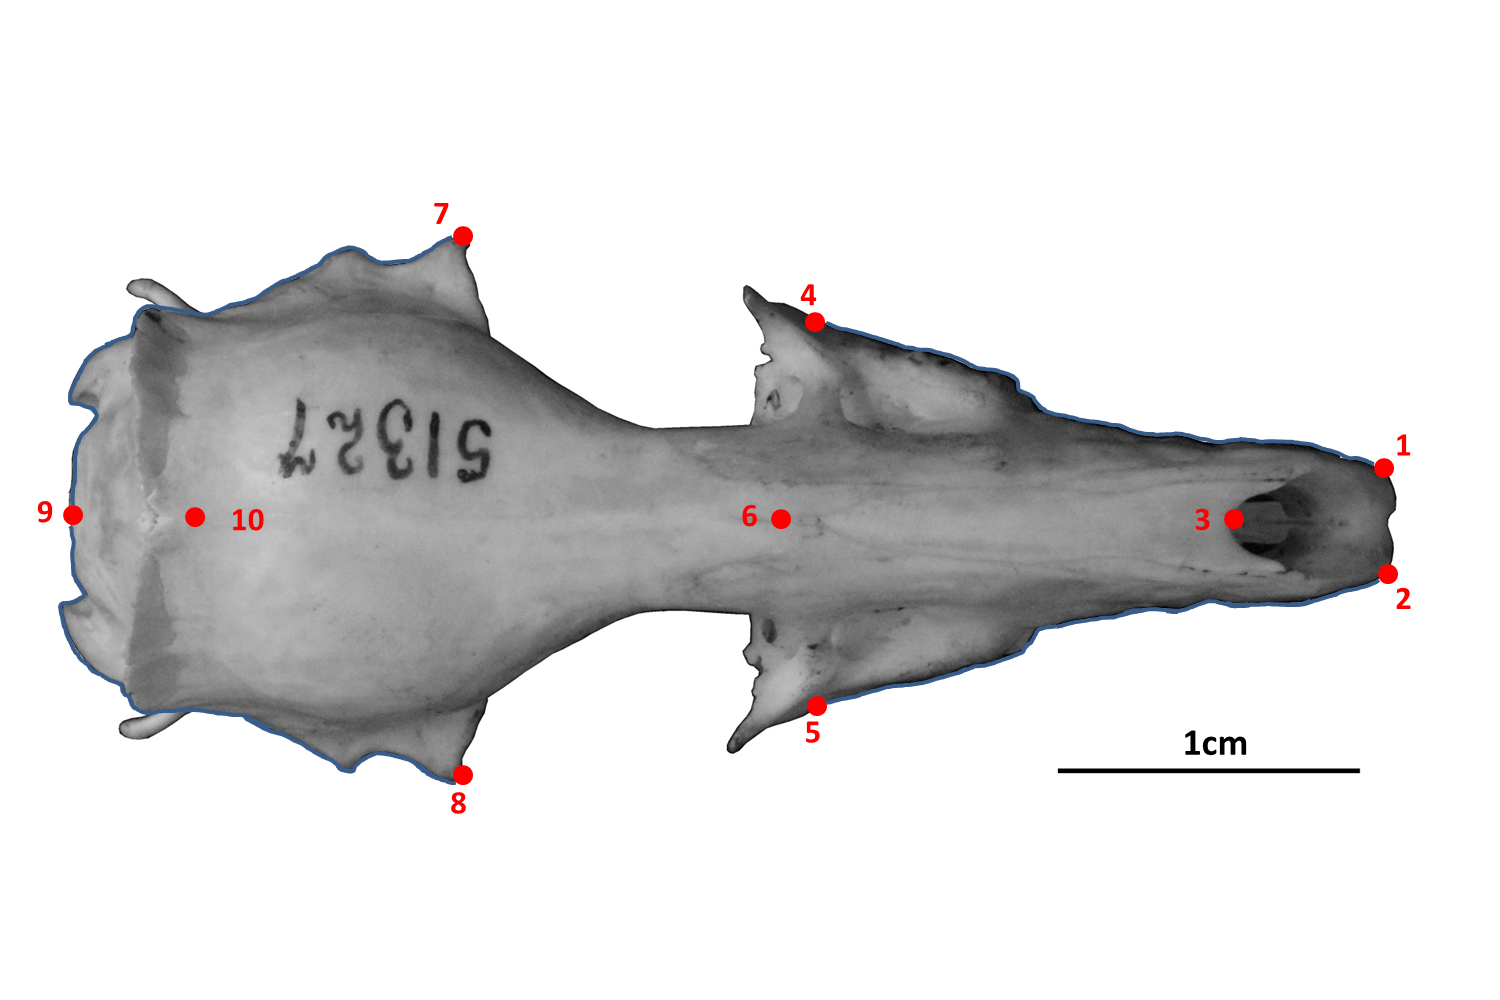
\includegraphics[width=1\linewidth]{Methods/figures/AMNH_51327_dorsallandmarksdiagram.png}
	\caption[Skulls: dorsal landmarks]
	{Landmarks (red) and curves (blue) for the skulls in dorsal view. Curves were re-sampled to the same number of evenly-spaced points. See table \ref{tab:skdors} for description of curves and landmarks.\textit{Potamogale velox} (Tenrecidae) skull, museum accession number: AMNH\_51327}
	\label{fig:skdors_landmarks}
\end{figure}


\begin{table}[h]
	\caption[Skulls: dorsal landmarks]
		{Descriptions of the landmarks (points) and curves (semilandmarks) for the skulls in dorsal view (figure
		\ref{fig:skdors_landmarks})} 
	%Skdors landmarks

\begin{tabular}[t]{p{3cm}  l}		
\hline
\textbf{Landmark} & \textbf{Description} \\
\hline
%------------------------------------------------------------
1 + 2 & Left (1) and right (2) anterior points of the premaxilla \\
%------------------------------------------------------------
3 & Anterior of the nasal bones in the midline \\
%------------------------------------------------------------
4 + 5 &	Maximum width of the palate (maxillary) on the left (4) and right (5)\\
%------------------------------------------------------------
6 & Midline intersection between nasal and frontal bones \\
%------------------------------------------------------------
7 + 8 & Widest point of the skull on the left (7) and right (8) \\
%------------------------------------------------------------
9 &	Posterior of the skull in the midline \\
	%Panchetti 2008 and Macholan2008 have different definitions for this one so I need to choose one
%------------------------------------------------------------
10 & Posterior intersection between saggital and parietal sutures \\
%--------------------------------------
\hline
\textbf{Curve A} & Outline of the braincase on the left side, between landmarks 9 and 7\\ 
(12 points) & (does not include visible features from the lower (ventral) side of the skull) \\

\textbf{Curve B} & Outline of the palate on the left side, between landamarks 4 and 1 \\
(10 points) & (outline of the rostrum only, not the shape of the teeth)\\

\textbf{Curve C} &	Outline of the braincase on the right side, between landmarks 9 and 8 \\
(12 points) & (does not include visible features from the lower (ventral) side of the skull) \\

\textbf{Curve D} & Outline of the palate on the right side, between landamarks 5 and 2 \\
(10 points) & (outline of the rostrum only, not the shape of the teeth)\\
%------------------------------------------------------------
\hline
\end{tabular}
	\label{tab:skdors}
\end{table}


%-------------------------------------------------------------
\subsection{\normalfont{Skulls: ventral view}}

	Most of the landmarks in this view are concentrated around the dentition and palate of the animals. I placed 13 landmarks and drew one outline curve (resampled to 60 semilandmark points) around the back of the skull between landmarks 12 and 13 (figure \ref{fig:skvent_landmarks}). The high variability of my species’ basi-cranial region and difficulties associated with identifying developmentally or functionally homologous points precluded designation of additional landmarks towards the back of the skulls. Table \ref{tab:skvent} outlines the descriptions of the landmarks I placed on the ventral pictures.

% Skulls ventral landmarks
\begin{figure}[!htb] 
  \centering
  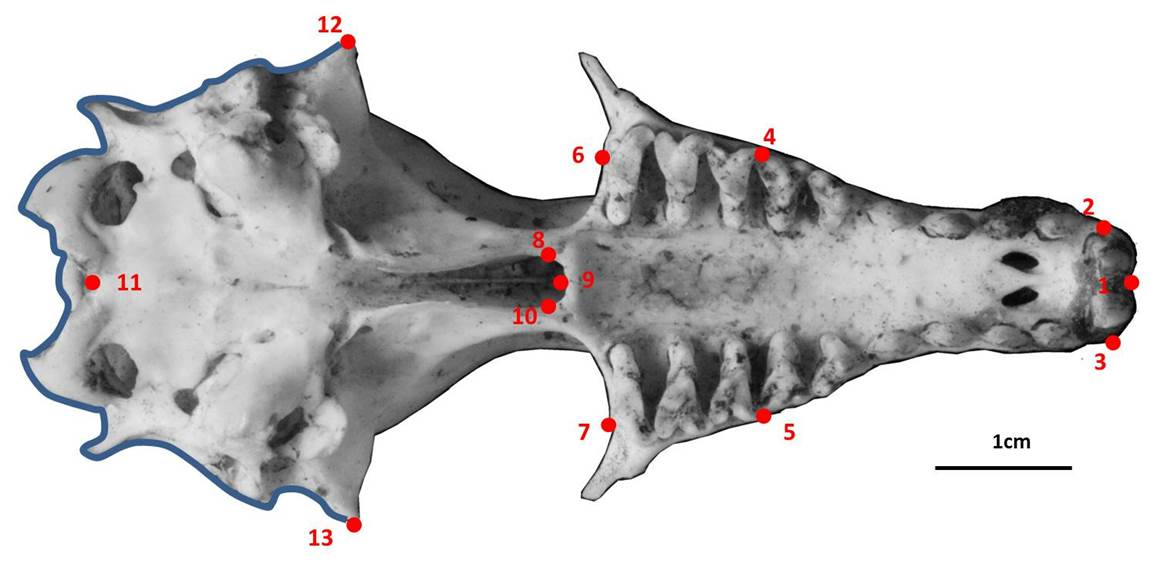
\includegraphics[width=12cm, height=12cm, keepaspectratio=true]{Methods/figures/skvent_landmarks_pot_vel.jpg}
    \caption[Skulls: ventral landmarks]
    {Landmarks (red) and curve (blue) for the ventral skull pictures, further descriptions in table \ref{tab:skvent}. The specimen is a giant otter shrew tenrec, \textit{Potamogale velox}, NHML 1934.6.16.2}
  \label{fig:skvent_landmarks}
  \end{figure}

\bigskip

\begin{table}[!htb] %force the table to go up with the picture
\caption[Skulls: ventral landmarks]
		{Descriptions of the landmarks (points) and curves (semilandmarks) for the skulls in ventral view (figure \ref{fig:skvent_landmarks})} 
%SkVent landmarks
\begin{tabular}[t]{p{0.2\textwidth} p{0.75\textwidth}}		
\hline
\textbf{Landmark} & \textbf{Description} \\
\hline
%--------------------------------------
1 & Anterior point of the palate\\
%--------------------------------------
2 + 3 & Posterior, lateral extremity of the right (2) and left (3) incisor\\
%--------------------------------------
4 + 5 & Anterior, outer point of the first molar on the right (4) and left (5)\\
%--------------------------------------
6 + 7 & Posterior, outermost point of the last molar surface on the right (6) and left (7) \\
%--------------------------------------
8 & Widest point of the curve of the palatine on the right side\\
%--------------------------------------
9 & Posterior point of the palatine in the midline\\
%--------------------------------------
10 & Widest point of the curve of the palatine on the left side\\
%--------------------------------------
11 & Anterior of the occipital foramen in the midline\\
%--------------------------------------
12 + 13 & Widest (extreme lateral) point of the braincase on the right (12) and left (13)\\
%--------------------------------------
Curve*  & Outline of the back of the skull (between landmarks 12 and 13), 60 points \\
%------------------------------------------------------------
\hline
\end{tabular}
\label{tab:skvent}
\end{table}
%----------------------------------------------------	
\newpage
\subsection{\normalfont{Skulls: lateral view}}
	I placed nine landmarks on the lateral pictures (see figure \ref{fig:sklat_landmarks} below) and also drew two semilandmark curves between landmarks 7 and 8 to represent the shape of the back of the skull (resampled to 20 semilandmark points) and landmarks 8 and 1 (resampled to 15 semilandmark points) down the midline of the nose to represent the shape of the top of the skull. Table \ref{tab:sklat} describes my definitions for each of the landmark points.
	If specimens that were damaged on their right side I reflected photographs of the left lateral side of the skull so that all pictures would be in the same orientation.
	I originally tried to include more landmarks around the infraorbital foramina (IF) as a crude measure of facial sensitivity and because the IF area is correlated with ecotypes \citep{Crumpton2012}. However, it proved impossible to see the boundaries of the IF in many species and single landmark points could not represent the shape of the full foramina. 

%Sklat diagram and landmarks description
\begin{figure}[!htb] 
  \centering
  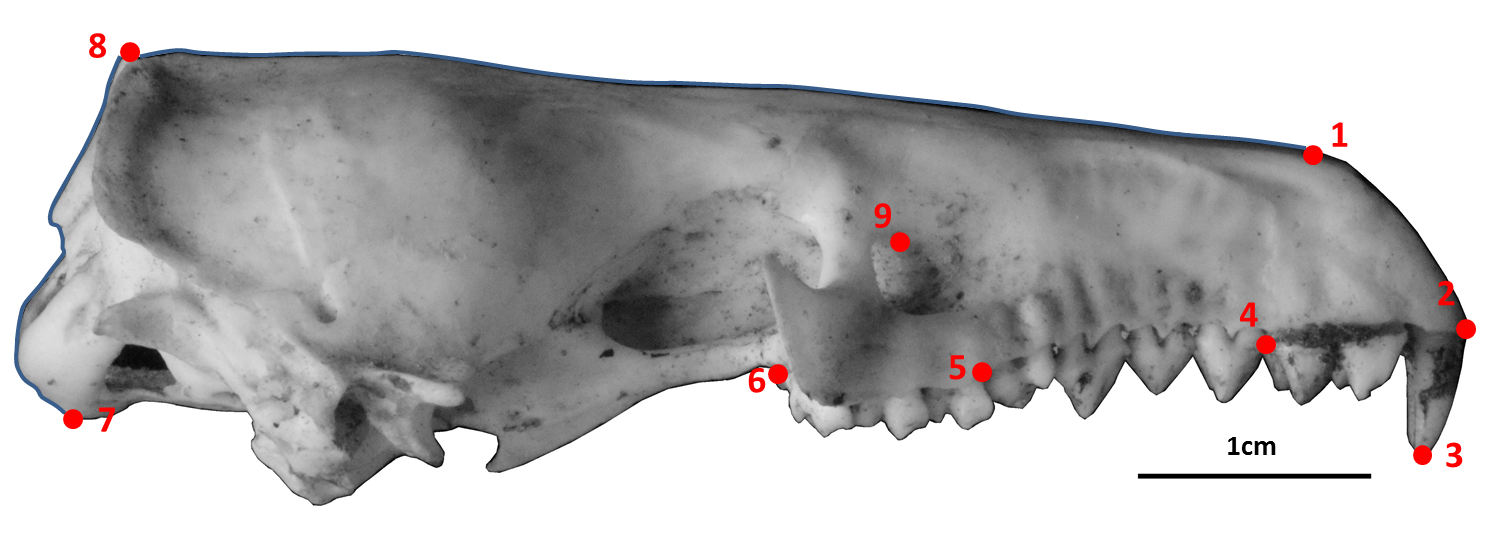
\includegraphics[width=12cm, height=12cm, keepaspectratio=true]
  {Methods/figures/sklat_landmarks_pot_vel.png}
    \caption[Skulls: lateral landmarks] {Landmarks (red) and curve (blue) for the lateral skull pictures, further descriptions in table \ref{tab:sklat}. The specimen is a giant otter shrew tenrec, \textit{Potamogale velox}, NHML 1934.6.16.2}
  \label{fig:sklat_landmarks}
  \end{figure}

\begin{table}[!htb]
\caption[Skulls: lateral landmarks]
		{Descriptions of the landmarks (points) and curves (semilandmarks) for the skulls in lateral view (see Figure X.} 
%Sklat landmarks

\begin{tabular}[t]{p{2cm} p{12cm}}		
\hline
\textbf{Landmark} & \textbf{Description} \\
\hline
%--------------------------------------
1 & Anterior, upper tip of the nasal bone\\
%--------------------------------------
2 & Anterior of the alveolus of the first incisor\\
%--------------------------------------
3 & Lowest point of the first incisor\\
%--------------------------------------
4& Posterior of the alveolus of the last incisor \\
%--------------------------------------
5 & Anterior tip of the alveolus of the first molar\\
%--------------------------------------
6 & Posterior tip of the alveolus of the last molar\\
%--------------------------------------
7 & Lowest point of the basi-occipital (base of the back of the skull)\\
%--------------------------------------
8 & Highest point of the braincase\\
%--------------------------------------
9 & Highest point of the infraorbital foramen\\
%--------------------------------------
\hline
\textbf{Curve A} & Between points 7 and 8  \\
(20 points)& Back of the skull from the lowest to highest points\\
%------------------------------------------------------------
\textbf{Curve B} & Between points 8 and 1  \\
(15 points)&From the highest point of the braincase to the front of the nasal \\
%------------------------------------------------------------
\hline
\end{tabular}
\label{tab:sklat}
\end{table}

%--------------------------------------------------------
\newpage
\subsection{\normalfont{Mandibles}}
	I placed seven landmarks and drew four curves on each mandible picture (again, reflecting any pictures of the left mandible so they could be compared to pictures of the right side). I drew separate curves around each of the three processes of the ascending ramus; coronoid, condyloid and angular and along the base of the horizontal ramus of the jaw. While obviously part of an integrated jaw unit, the development of the mandibular processes are also, in some aspects, independent since they attach different muscles which exert different masticatory forces on the jaw \citep{Barrow2008}. Therefore, by drawing separate curves around each of these elements, my ensuing analyses could assess the relative shape changes of different components of the jaw with relevance to variation in feeding strategies and capabilities.
	
	\newpage %Put's the next section onto a new page, not the figures and table
%********
%Why do we care about independence??
%I don’t like how I’ve phrased the above paragraph but I just thought it was a nice point in the Barrow paper so I want to include it somewhere.
%********

%Mandibles' landmarks
\begin{figure}[!htb]
	\centering
	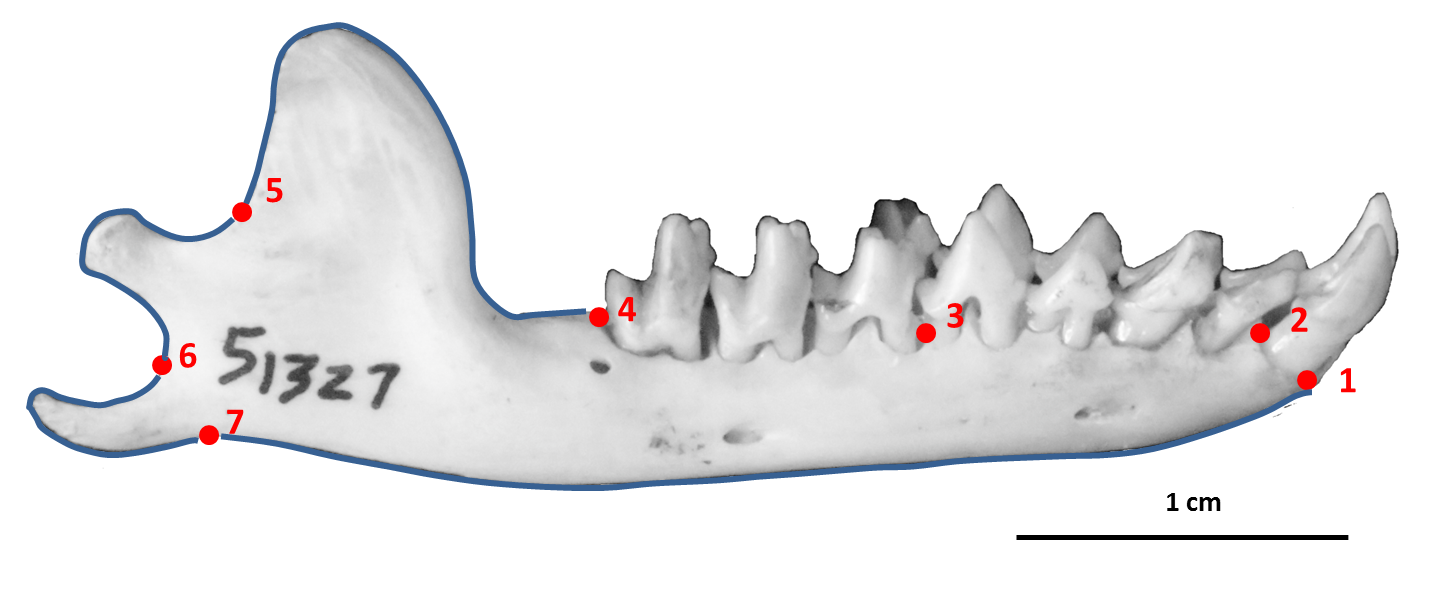
\includegraphics[width=1\linewidth]{Methods/figures/AMNH_51327_landmarksdiagram.png}
	\caption[Mandibles' landmarks]
			{Landmarks (red) and curves (blue) used for the mandibles. Curves were re-sampled to the same number of evenly-spaced points. See table \ref{tab:mands} for description of curves and landmarks.\textit{Potamogale velox} (Tenrecidae) mandible, accession number: AMNH\_51327}
	\label{fig:mands_landmarks}
\end{figure}

\begin{table}[!htb]			
	\centering
	\caption[Mandibles' landmarks]
		{Descriptions of the landmarks (points) and curves (semilandmarks) for the mandibles in lateral (buccal) view (figure \ref{fig:mands_landmarks}}
	%Mandibles landmarks


\begin{tabular}[t]{p{0.2\textwidth} p{0.75\textwidth}}		
\hline
\textbf{Landmark} & \textbf{Description} \\
\hline
1 & Anterior of the alveolus of the first incisor \\
2 & Posterior of the alveolus of the first incisor \\
3 &	Anterior of the alveolus of the first molar \\
4 & Posterior of the alveolus of the last molar \\
5 & Maximum curvature between the coronoid and condylar processes\\
6 & Maximum curvature between the condylar and angular processes  \\
7 &	Maximum curvature between the angular process and the horizontal ramus \\
%---------------------------------------------------
\hline
Curve A & Condyloid process (between landmarks 4 and 5, 15 points)\\
Curve B & Condylar process (between landmarks 5 and 6, 15 points) \\
Curve C & Angular process (between landmarks 6 and 7, 15 points)  \\
Curve D & Base of the jaw (between landmarks 7 and 1, 12 points)  \\
%---------------------------------------------------
\hline
\end{tabular}
	\label{tab:mands} 
\end{table}
%-----------------------------------------------

\section{Procrustes superimposition}
\label{sect:procrustes}

	After creating my files with the landmarks and semilandmarks placed on each picture, I used TPSUtil \citep{Rohlf2012} to create sliders files \citep{Zelditch2012} to define which points were semilandmarks. I conducted all further morphometric analyses in R version 3.1.1 \citep{Team2014} within the geomorph package \citep{Adams2013}.
	For each of the separate data sets, we used the gpagen function to run a general Procrustes alignment \citep{Rohlf1993} of the landmark coordinates while sliding the semilandmarks by minimising procrustes distance \citep{Bookstein1997}.
	We used these Procrustes-aligned coordinates of all specimens to calculate average shape values for each species which we then used for a principal components (PC) analysis with the plotTangentSpace function \citep{Adams2013}. 


%####################################################

%I'm not sure whether this is the most appropriate way to deal with errors: I could split up the sections and put them at the end of each of the previous sections rather than breaking up the story here but that might be more fragmented overall

\section{Error checking}
\label{sect:errors}
	My data are prone to a number of different error sources. These include 1) taxonomic identification which has not been updated to currently accepted terms, 2) specimen ID errors, 3) possible variation associated with sex and age class of individuals, 4) the accuracy and repeatability with which species traits are measured, 5) morphometric errors associated with photographing specimens and the placement of landmarks. I address each of these possible sources of error below.  

\subsection{\normalfont{Taxonomic}}
	I recorded species names as they were written on museum specimen labels and then corrected them to match the taxonomy in Wilson and Reader’s Mammal Species of the World \citeyearpar{Wilson2005}. For recently identified species, such as \textit{Microgale jobihely} \citep{Goodman2006}, which are not included in Wilson and Reader \citeyearpar{Wilson2005}, I used the taxonomy recorded on the labels. 

\subsection{\normalfont{Specimen ID}}
	%add in Natalie's centroid means?
	
	There were four specimens from the Smithsonian Institute that had species labels which did not match between skulls and skins with the same specimen ID numbers. The four skulls were labelled as \textit{Hemicentetes semispinosus}. The corresponding skins were originally labelled as \textit{H. semispinosus} but this was crossed out and changed to \textit{H. nigriceps}. The re-labelled skins looked clearly different to the undisputed \textit{H. semispinosus} skins and also look more similar to other pictures of \textit{H. nigriceps}. Therefore, I made the assumption that the re-labelling of the skins as \textit{H. nigriceps} represents the true taxonomy and I treated the corresponding skulls as \textit{H. nigriceps}.

\subsection{\normalfont{Specimen sex and age}}


	Information about the sex and/or age of an individual is often missing from museum records. Mammalian species can often be identified as juveniles by looking for incomplete fusion of the crania and non-fully erupted dentition (REFS) However, age classification in tenrecs is difficult using these criteria; in some species, the last molar does not erupt fully until the first molar has been shed so the full dentition is never present at any one time \citep{Nowak1983}. It is also difficult to distinguish deciduous from permanent teeth in \textit{Microgale} tenrecs \citep{Asher2008} which has led to confusion and misidentification of juvenile forms as separate species \citep{Olson2004}. I excluded any obvious juvenile specimens from my data set. Where specimens could not be obviously identified as juveniles I treated them all as equivalent adult forms. 	
	I included both male and female specimens in my data as significant sexual dimorphism in skull or body size has not been identified in any of my species \citep[REFS][]{Olson2004}.


\subsection{\normalfont{Linear measurements}}
	%Maybe this isn't relevant anymore since I'm not actually doing anything with the linear measurement data?
	As mentioned above (section \ref{sect:measurements}), I took three replicate measurements of most of my variables and five replicates of other variables. 
	Some morphometric studies take replicate measurements of a trait and use the average value for further analyses (REFS). Rather than taking the mean of each of three (or five) measures, I used the median as it is less likely to be skewed by outliers and gives a more accurate representation of the true value of the trait (REFS?).
	Before extracting the median values I followed the protocol for assessing measurement error outlined by \citep{Cooper2009}. This method assesses whether there is a reasonable correlation among the replicate measurements of the same variable. The error checking criteria are based on two calculations; the coefficient of variation and the percentage spread.
	
	I calculated the coefficient of variation (standard deviation/mean*100) for each measurement. This value estimates the extent to which replicate measurements deviate from the mean. When the coefficient of variation was less than 5\%, I accepted the median value as an accurate measurement of the size of the structure. 
	If the coefficient of variation was greater than 5\%, indicative of a low agreement between replicate measurements, I measured the percentage spread of the data. For variables measured three times, I calculated percentage spread as [(minimum difference between neighbouring measurements)/ (range of measured values)*100].
	For variables that I measured five times, the differences between neighbouring values were calculated and labelled from smallest to largest as a, b, c, and d with the range of the measured values designated as e \citep{Cooper2009}. For these variables, I calculated percentage spread as [(a/e + b/e + c/e)*100]. 
	Small percentage spread values indicate close agreement between repeated measurements. When percentage spread approaches 50\% the data are evenly spread out and therefore there is no way of knowing whether the median value is an accurate measurement of the trait \citep{Cooper2009}. I chose to use to use 25\% as a cut off point for accepting the accuracy of measured traits.

	I used these error checking criteria to assess the accuracy of my repeated measurements of both skulls and limbs. 

%I've taken this out for now since I'm not actually using any of the linear measurement data
	%Of the 20 measurements for xxx skulls, there were xx variables belonging to xx skulls which had coefficient of variation > 5\% and percentage spread >25 \%. My final skull data set included xx replicates of xx variables from xx specimens comprising xx species.

	%Of the 19 measurements for xxx limbs, there were xx variables belonging to xx specimens which had coefficient of variation > 5\% and percentage spread >25 \%. My final limb data set included xx replicates of xx variables from xx specimens comprising xx species.

\subsection{\normalfont{Potential morphometrics error}}

	I used 2D morphometrics to compare the morphologies of the skulls (section \ref{sect:morphometrics}). The small size of my specimens, combined with the number of specimens involved in my study made 3D imaging impractical. It takes roughly 1.5 hours for a good quality scan of each specimen so it would have taken me at least 550 hours to scan the 366 specimens that I photographed.
	 
	While 2D methods are an accepted means of comparing morphological shape \citep[e.g.][]{Adams2004, Mitteroecker2009}, particularly for comparing skull morphologies of small mammals \citep[e.g.][]{Cardini2003, Panchetti2008, White2008, Barrow2008, Scalici2011}, the inherent discrepancies associated with comparing three dimensional objects using two dimensional pictures do introduce some difficulties of possible distortion of the image \citep{Arnqvist1998}. Similarly, human error with how landmarks are positioned on specimens could also introduce noise into further analyses. 
	In contrast to detailed intraspecific work (REFS) photographic or landmark placement errors are unlikely to be significant in interspecific studies since one would expect that the morphological variation among species is large enough to  be detected as a signal above any background noise associated with methodological error (REFS). Nevertheless, it is still important to assess measurement error in a morphometric data set to increase confidence in the outcome of final analyses.
	I identify two main sources of morphometric measurement error; specimen orientation and placement of landmarks.

	%***************************
	%NB: I never actually completed these error checking analyses so I need to go back and do it again if I am going to include it
	%********************************

	Variation in the orientation of specimens for photography is one of the main sources of error in 2D morphometric studies \citep{Adriaens2007}. If specimens are not placed on a flat plane or in a consistent position relative to the camera, areas of the object which are tilted towards the camera will appear to be larger than reality, distorting any subsequent morphometric analyses of the shape. 
	I used a random subset of skulls comprised of one representative from each of my 89 species %(probably don’t need to use this many for error checking but how should I choose which ones to include?) 
	to estimate the overall specimen orientation error in my photographic dataset. This subset included representatives from each tenrec and golden mole species along with samples from my comparative species (total of xx moles, xx shrews, xx hedgehogs ...)  I took three sets of pictures of each view of the skulls and mandibles, cycling through the pictures so that the specimen was removed and re-positioned before every shot \citep{Viscosi2011}. 
	%********I need to add more here if I come back to do these analyses

\subsection{\normalfont{Landmark placement}}

	I placed the landmarks on each set of pictures so inter-observer variation is not an issue for my study.  However, repeatability and reliability of my choice of landmarks could affect the final results of my analyses \citep{Arnqvist1998}.
	I used a combined, nested approach to test for both orientation and landmark placement error \citep{Arnqvist1998, Barrow2008}. For each of the 89 specimens in my random subset of species, I photographed their skulls (dorsal, ventral and lateral views) and mandibles three times. I then copied these images and placed landmarks on 3 copies of each image. I used a nested mixed mode ANOVA to assess the measurement error of the Procrustes-superimposed coordinates. There were three factors in my ANOVA; specimen, photo (3 pictures of each specimen) and landmark trial (placed landmarks on 3 copies of each of my photos).


	%Effect size for the variance explained by each factor, based on inter landmark linear distances……..
	%(I could also use PC scores or a Mahalanobis distance matrix…)

%#########################################################
%DATA ANALYSES
%##################################################
\section{Data Analysis}
\label{sect:data_analysis}

Introduction to the data analyses

\subsection{\normalfont{Comparing tenrecs' diversity to their closest relatives}}
%I copied most of this section from the methods part of my disparity paper

	For each of the morphometric data sets (dorsal, ventral, lateral skulls and mandibles), I ran a general Procrustes alignment (section \ref{sect:procrustes}) of just my tenrec and golden mole specimens to compare morphological diversity in the two families. I used the principal components axes which accounted for 95 \% of the cumulative variation to calculate four disparity metrics; the sum and product of the range and variance of morphospace occupied by each family \citep{Brusatte2008, Foth2012, Ruta2013}. We also calculated morphological disparity directly from the Procrustes-superimposed shape data based on the sum of the squared inter-landmark distances among species pairs \citep[SSqDist,][]{Zelditch2012}.
	
	I used two approaches to test whether tenrecs have significantly different morphologies compared to golden moles. The first was a comparison of morphospace occupation between the two groups with non parametric MANOVAs \citep{Anderson2001} to test whether tenrecs and golden moles occupy significantly different areas of morphospace \citep[e.g][]{Serb2011, Ruta2013}. 
	
	Secondly, I used pairwise permutation tests to test the null hypothesis that tenrecs and golden moles have equal disparity. If this hypothesis were true then the designation of each species as belonging to either tenrecs or golden moles should be arbitrary because each group would have the same disparity. Therefore I permutated the data by assigning family identities at random to each specimen and calculated the differences in disparity for each of the new family groupings. I repeated these permutations 1000 times to generate a null distribution of the expected differences in family disparity. I compared the observed (true) measures of the differences in disparity between tenrecs and golden moles to these permutated distributions to test whether the families had significantly different levels of disparity.

	The majority of tenrec species (19 out of 31 in my data) are members of the \textit{Microgale} (shrew-like) genus which is notable for its relatively low phenotypic diversity \citep{ Soarimalala2011, Jenkins2003}. The strong similarities among these species may mask signals of higher disparity among other tenrecs. Therefore I repeated my family-level comparisons of disparity with a reduced data set that excluded the \textit{Microgale} so that I could compare disparity within the remaining 12 tenrec species to disparity within the 12 species of golden moles.



\subsection{\normalfont{Quantifying convergence among tenrecs and other small mammals}}


%Phylogeny section from the original disparity paper; probably relevant when I go back to the convergence analyses

\subsubsection{Phylogeny} % I still have the problem of subsubsections not getting numbered in the main text
	Instead of basing my analyses on individual trees and assuming that their topologies are known without error \citep[e.g.][]{Ruta2013, Foth2012, Brusatte2008, Harmon2003} I used a distribution of 101 pruned phylogenies derived from the randomly resolved mammalian supertrees in \citep{Kuhn2011}. 
		% I used 101 because that was the number in the smaller Fritz file - I could change it to 100 instead if 101 sounds odd?

	Eight species (six \textit{Microgale} tenrecs and two golden moles) in my morphological data sets were not in the phylogenies. Phylogenetic relationships among the \textit{Microgale} have not been resolved more recently than the \citep{Kuhn2011} analysis, therefore I added the additional \textit{Microgale} species at random to the \textit{Microgale} genus within each phylogeny \citep{Revell2012}. I could not use the same approach to add the two missing golden mole species because they were the only representatives of their respective genera within my data. Therefore I randomly added these species to the common ancestral node (using the findMRCA function in phytools \citep{Revell2012}) of all golden moles within each phylogeny. Adding these extra species to the phylogenies created polytomies which I resolved arbitrarily using zero-length branches \citep{Paradis2004}. I calculated pairwise phylogenetic distances among species using the cophenetic function \citep{Team2014}. 





	
\chapter{Morphological diversity in tenrecs compared to golden moles}
\label{chap:disparity}


\section{Introduction}
	In Chapter \ref{chap:introduction}, I explained why it is important to study patterns of morphological diversity in tenrecs. In this chapter, I present the first quantitative investigation of morphological diversity in tenrecs. I use geometric morphometric techniques \citep{Rohlf1993} to compare cranial morphological diversity in tenrecs to that of their closest relatives, the golden moles. 
	I expect tenrecs to be more morphologically diverse than golden moles because tenrecs occupy a wider variety of ecological niches. The tenrec Family includes terrestrial, semi-fossorial, semi-aquatic and semi-arboreal species \citep{Soarimalala2011}. In contrast, all golden moles occupy very similar, fossorial ecological niches \citep{Bronner1995}. 
	Greater ecological variety is often (though not always) correlated with higher morphological diversity \citep{Losos2010a}. In this chapter I test whether this prediction is supported when I compare morphological diversity in tenrecs to golden moles.

%------------------------------------------------------
\section{Methods}

	The methods I used to measure morphological diversity involved several steps of data collection, processing and analysis. For clarity,  Figure \ref{fig:flow} summarises all of these steps and I describe them in detail below. Note that I repeated the same analyses for each of the different sets of photographs: skulls in dorsal, ventral and lateral views, and mandibles in lateral view.
	
%*************************************************
%Methods flowchart: 
%**************************************
	%SF: I've changed parts of this compared to the chart in the paper manuscript but the overall steps are the same because I'm hoping that the new description in the text makes them clearer.
		\begin{figure}[!htbp]
		\centering
		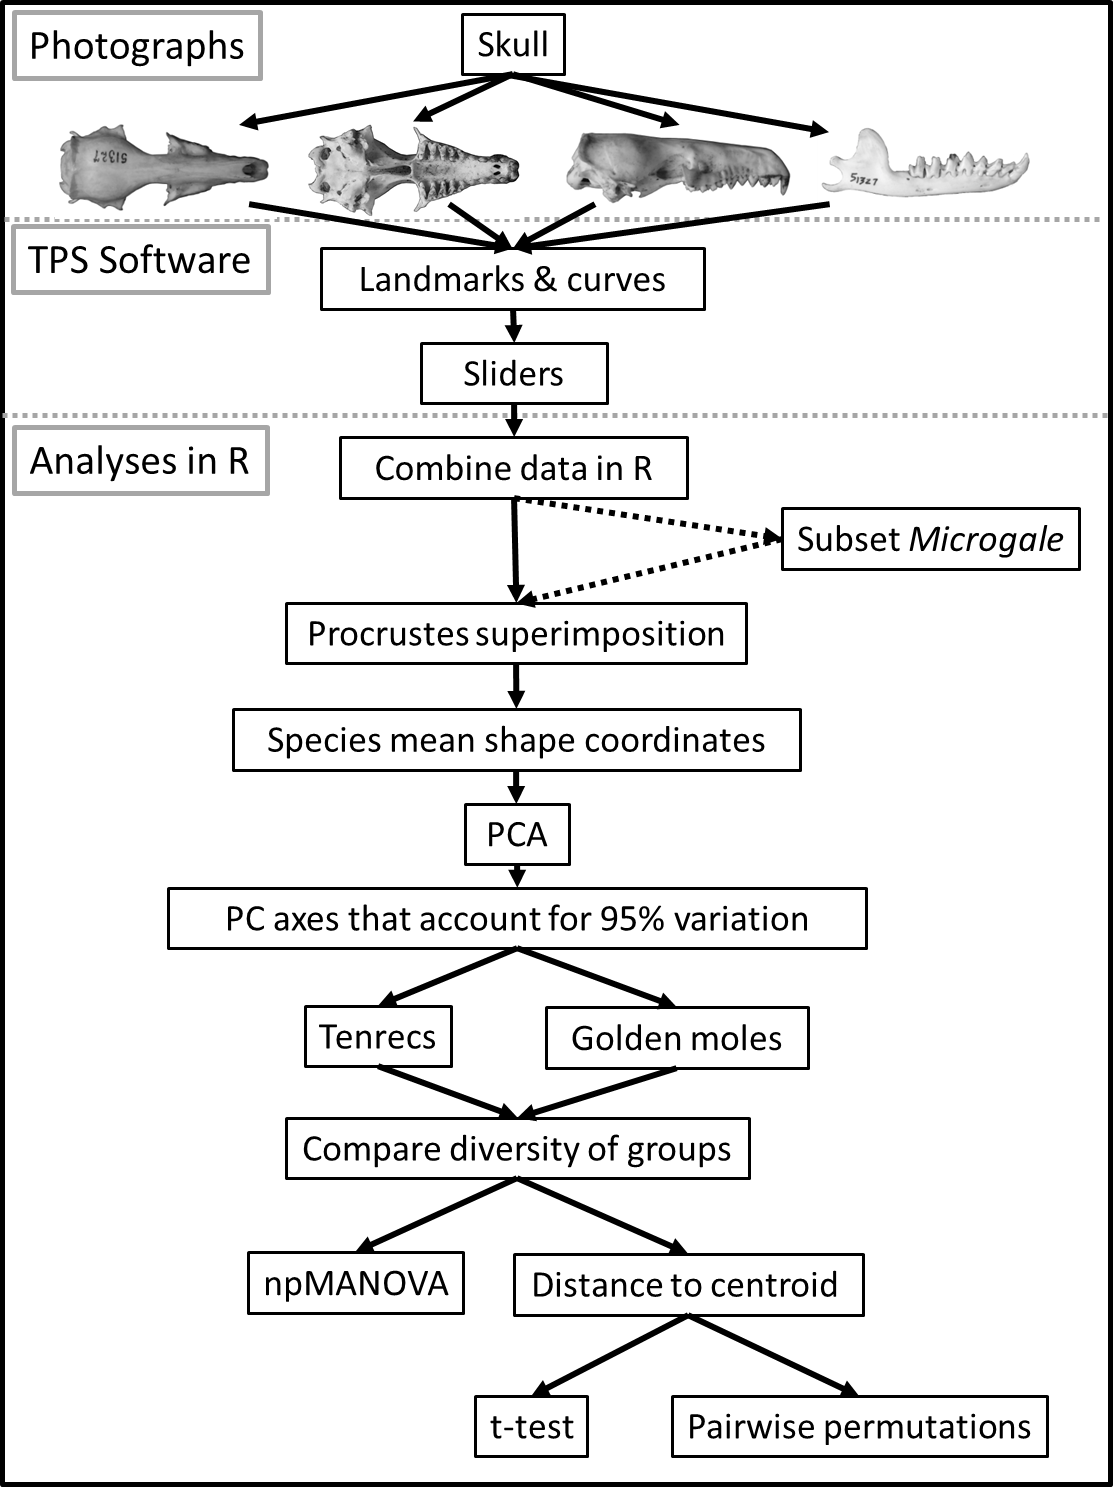
\includegraphics[width=1\linewidth,height=0.8\textheight]{Disparity/writing/figures/Methods_flowchart_thesis.png}
		
		\caption[Flowchart diagram of data collection and analysis]
			{Summary of the main steps in my data collection, processing and analysis protocol. Note that the analyses were repeated separately for each set of photographs: skulls in dorsal, ventral and lateral views and mandibles in lateral view. The dashed arrows refer to the stage at which I selected a subsample of the tenrecs (including just five species of the \textit{Microgale} Genus) so that I could compare the morphological diversity of this reduced subsample of tenrec species to the diversity of golden moles.}
		
		\label{fig:flow}
		\end{figure}
%----------------------------------------------------	

	In Chapter \ref{chap:methods} (Figure \ref{fig:flow}), I described how I photographed skulls and summarised their morphologies using landmark morphometrics. I used photographs of 182 skulls in dorsal view (148 tenrecs and 34 golden moles), 173 skulls in ventral view (141 tenrecs and 32 golden moles), 171 skulls in lateral view (140 tenrecs and 31 golden moles) and 181 mandibles in lateral view (147 tenrecs and 34 golden moles). These samples represent 31 species of tenrec (out of the total 34 in the Family; \citealp{Olson2013}) and 12 species of golden moles (out of a total of 21 species in the Family; \citealp{Asher2010}). Note that the number of skulls I used varies slightly for each analysis because some skulls were damaged in certain views.
	

	After placing the landmarks and creating sliders files within the TPS software series (Chapter \ref{sect:morphometrics}, Figure \ref{fig:flow}), I combined the files into a single morphometrics data object and carried out all further analyses in R version 3.1.1 \citep{Team2014} and my code is available on GitHub \citep{Finlay2015c}. At this stage, I either used the full data set (31 species of tenrec and 12 species of golden mole) or a reduced data set with just 17 species of tenrec. I created this reduced data set because the majority of tenrec species (19 out of 31 in my data) belong to the \textit{Microgale} (shrew-like) Genus that has relatively low morphological diversity \citep{Soarimalala2011, Jenkins2003}. This may mask signals of higher morphological diversity among other tenrecs. In contrast, species richness across Genera within the golden mole phylogeny is more evenly distributed (see Appendix \ref{phylo}). To test this, I created a subset of the tenrec data that included just five of the \textit{Microgale} species, each representing one of the five sub-divisions of \textit{Microgale} outlined by Soarimalala and Goodman \citeyearpar{Soarimalala2011}, i.e. small, small-medium, medium, large and long-tailed species. I compared the morphological diversity of this subset of tenrecs (n=17: five \textit{Microgale} and 12 non-\textit{Microgale} species) to that of the 12 species of golden moles (dashed arrows in Figure \ref{fig:flow}). After this selection stage, all further steps in the analyses were the same.
		
	For each analysis, I did a general Procrustes alignment of the shape data and calculated the mean shape coordinates for every species (see section \ref{sect:procrustes}). I used these average, Procrustes-superimposed shape coordinates for a principal components analysis (PCA) and then selected the number of principal component (PC) axes that accounted for 95\% of the variation in the data (Figure \ref{fig:flow}). Selecting the number of PC axes based on their cumulative variance \citep[e.g.][]{Brusatte2008, Collar2006} rather than through an arbitrary cut off standardised my diversity comparisons across the different analyses.
	
\subsection{\normalfont{Estimating morphological diversity}}
	
	I grouped the PC scores for tenrecs and golden moles separately so that I could estimate the diversity of each Family and then compare the two groups (Figure \ref{fig:flow}). I compared morphological diversity in two ways. First, I used non parametric multivariate analysis of variance \citep[npMANOVA;][]{Anderson2001} to test whether tenrecs and golden moles occupied significantly different positions within the morphospaces defined by the PC axes that accounted for 95\% of the overall variation in the data \citep[e.g.][]{Serb2011, Ruta2013}. A significant difference between the two Families would indicate that they have unique morphologies which do not overlap. Second, I compared morphological diversity within tenrecs to the diversity within golden moles. I define morphological diversity as the mean Euclidean distance (sum of squared differences) between each species and its Family centroid (Figure \ref{fig:centroids}). This is summarised in the equation below where \textit{n} is the number of species in the Family, \textit{i} is the number of PC axes and \textit{c} are the average PC scores for each axis (the centroid). 
	
	\begin{equation}
	Diversity = \frac{\sqrt{\Sigma(PCn_{i}-PCc_{i})^2}}{n}
	\end{equation}

	
	
	If tenrecs are more morphologically diverse than golden moles, then they should be more dispersed within the morphospaces and have, on average, higher values of mean Euclidean distance. 
	

%-----------------------------
%Diagram of mean distance to centroid (based on the diagram in Cooper et al 2009)
	\begin{figure}[!htbp]
	\centering
	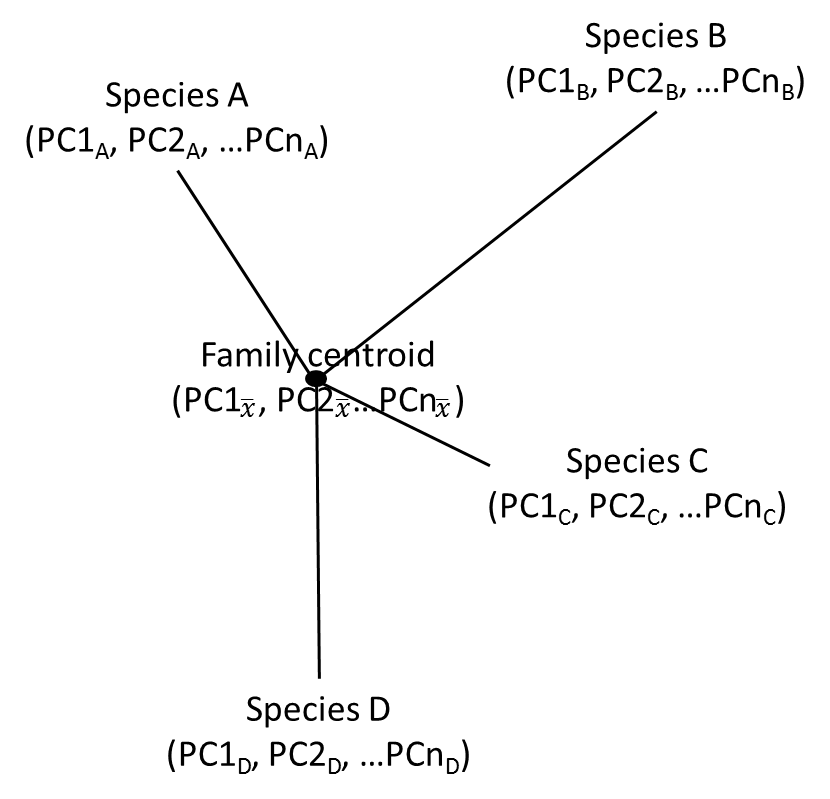
\includegraphics [width=0.7\linewidth, height=0.7\textheight, keepaspectratio]{Disparity/writing/figures/Centroids.png}
	\caption[Calculating diversity as mean Euclidean distance to Family centroid.]
		{Estimating morphological diversity as the mean Euclidean distance between each species and the Family centroid. Every species had scores on the principal components (PC) axes that accounted for 95\% of the variation in the principal components analysis. The number of axes (PCn) varied for each analysis but they were the same within a single analysis. PC scores were used to calculate the Euclidean distance from each species to the Family centroid (average (\begin{math}
			\bar{x}
			\end{math}) PC scores for the entire Family). Morphological diversity of the Family is the average value of these Euclidean distances.}
	\label{fig:centroids}
	\end{figure}
% SF: I moved the text and made the lines into double headed arrows, the error bar-type endings looked messy	

%--------------------------------------

	
	One possible issue with these analyses is that the two Families have unequal sample sizes: 31 (or a subset of 17) tenrec species compared to just 12 golden mole species. Morphological diversity is usually decoupled from taxonomic diversity \citep[e.g.][]{Ruta2013, Hopkins2013} so larger groups are not necessarily more morphologically diverse. However, comparing morphological diversity in tenrecs to the diversity of a smaller Family could still bias the results: overall diversity in tenrecs could be higher if diversity is simply a function of sample size. As described in the paragraph below, I used pairwise permutation tests to account for this potential issue. 

	I tested the null hypothesis that tenrecs and golden moles have the same morphological diversity (the same mean Euclidean distance to the Family centroid). If this is true, when you randomly assign the group identity of each species (i.e. shuffle the "tenrec" and "golden mole" labels) and then re-compare the morphological diversity of the two groups, there will be no significant difference between these results and those obtained when the species are assigned to the correct groupings. 
	% NC: I've rephrased this as really what is happening here is that there is no difference between the results you get with proper groupings versus random groupings. You expect that random groupings give no difference.
	I performed this shuffling procedure (random assignation of group identity) 1000 times and calculated the difference in morphological diversity between the two groups for each permutation. This generated a distribution of 1000 values which are calculations of the differences in morphological diversity under the assumption that the null hypothesis (equal morphological diversity in the two Families) is true. This method automatically accounts for differences in sample size because shuffling of the group labels preserves the sample size of each group: there will always be 12 species labelled as "golden mole" and then, depending on the analysis, either 31 or 17 species labelled as "tenrec". Therefore, the 1000 permuted values of differences in morphological diversity create a distribution of the expected difference in diversity between a group of sample size 31 (or 17 in the case of the subsetted tenrec data) compared to a group of sample size 12 under the null hypothesis that the two groups have the same morphological diversity. I compared the observed measures of the differences in morphological diversity between the two Families to these null distributions to determine whether there were significant differences after taking sample size into account (two-tailed t test).
	
%----------------------------------------------------

\section{Results}
\label{sect:results}

	Figure \ref{fig:FourPCA} depicts the morphospaces defined by the first two principal component (PC) axes from my principal components analyses (PCAs) of skull and mandible morphologies. The PCAs are based on the average Procrustes -\\superimposed shape coordinates for skulls in three views (dorsal, ventral and lateral) and mandibles in lateral view.

%-----------------------------
% SF: I took away the silhouette legend
	
%PCA figure
	%From the twofamily_disparity_PCAplots script
	\begin{figure}[!htbp]
	\centering
	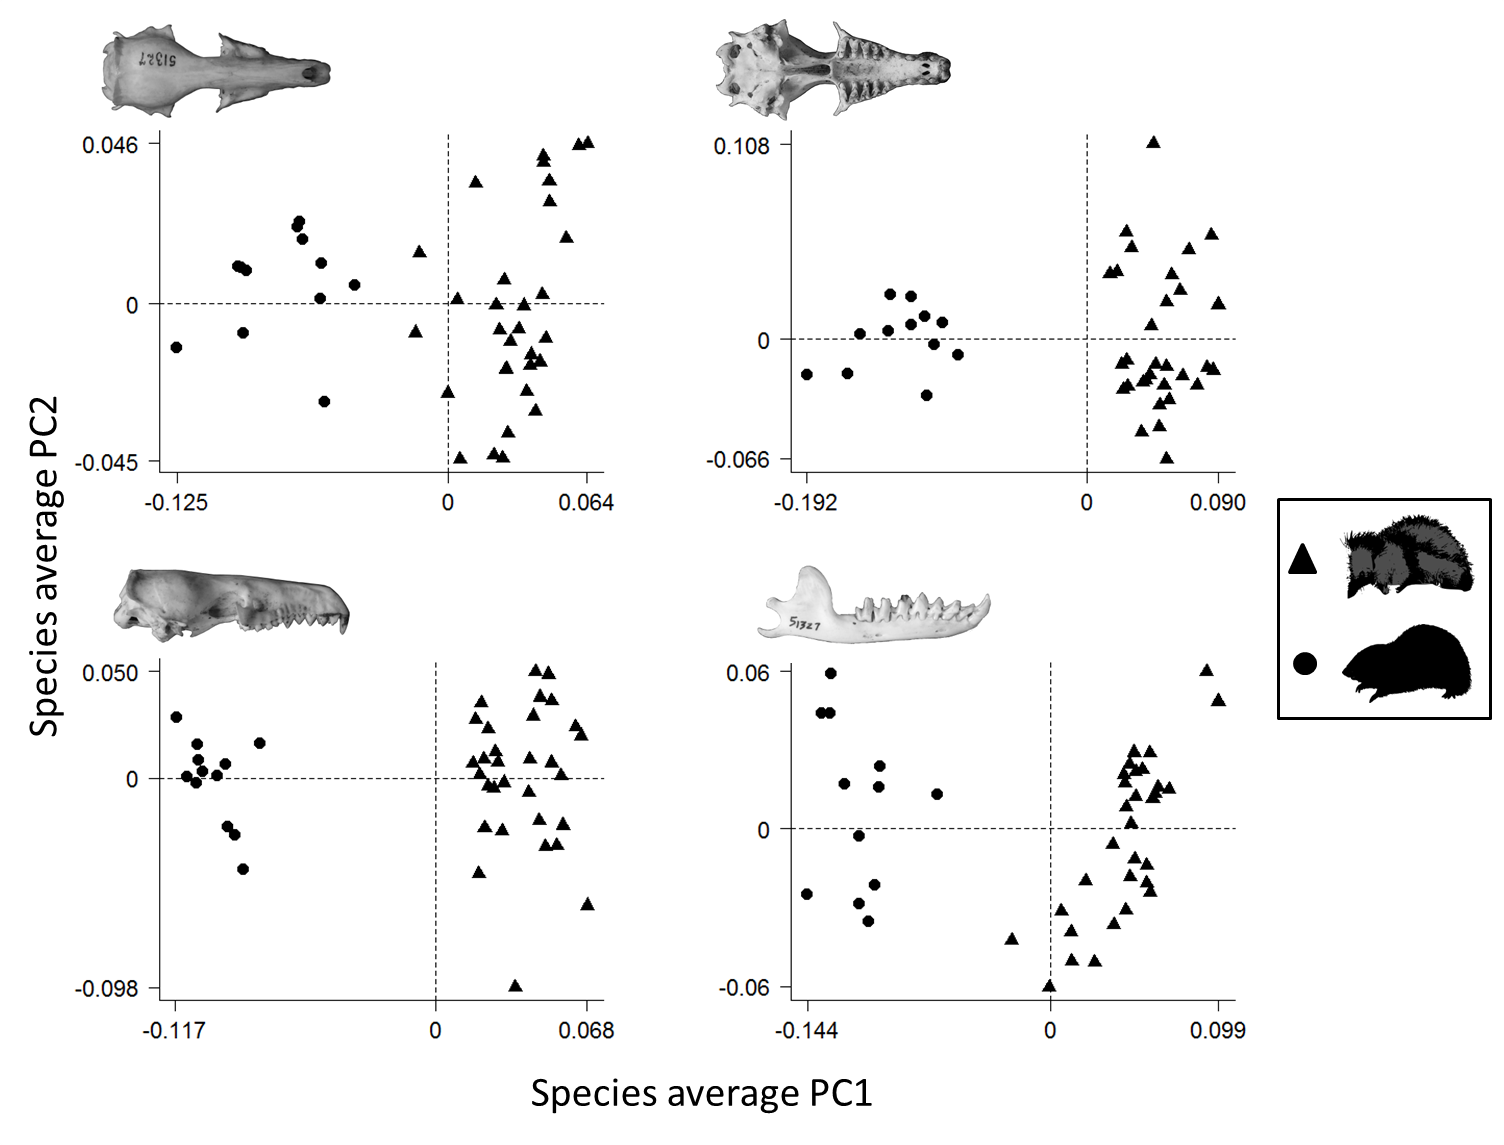
\includegraphics[width=1\linewidth, height=1\textheight, keepaspectratio]{Disparity/writing/figures/FourPCA_shapes.png}
	\caption[Morphospace (principal components) plot of morphological diversity in tenrec and golden mole skulls.]
		{Principal components plots of the morphospaces occupied by tenrecs (triangles, n=31 species) and golden moles (circles, n=12 species) for the skulls in dorsal (top left), ventral (top right) and lateral (bottom left) views, and mandibles in lateral view (bottom right). Each point represents the average skull shape of an individual species. Axes are principal component 1 (PC1) and principal component 2 (PC2) of the average scores from principal components analyses of mean Procrustes shape coordinates for each species.}
	\label{fig:FourPCA}
	\end{figure}
%----------------------------------------------

	To compare morphological diversity in the two families, I used the PC axes which accounted for 95\% of the cumulative variation in each of the skull analyses: dorsal (n=6 axes), ventral (n=7 axes) and lateral (n=7 axes) and the mandibles (n=11 axes). First, I compared the position of each Family within the morphospace plots. Tenrecs and golden moles occupy significantly different positions in the dorsal (npMANOVA: F\textsubscript{1,42}=68.13, R$^2$=0.62, p=0.001 ), ventral (npMANOVA: F\textsubscript{1,42}=103.33, R$^2$=0.72 , p=0.001 ) and lateral (npMANOVA: F\textsubscript{1,42}=76.7, R$^2$ =0.65, p=0.001 ) skull morphospaces as well as in the mandible morphospace (npMANOVA: F\textsubscript{1,42}=60.38, R$^2$=0.59, p=0.001),  indicating that the Families have very different, non-overlapping cranial and mandible morphologies (Figure \ref{fig:FourPCA}). 

	
	%SF: I changed the text to have no spacing around = and the tables have spaces around the +/- because otherwise it looks too cluttered
	
	%Numbers are from the npMANOVA based on PC axes within my diversity_twofamily_cent_dist script
%----------------------------------------
%Results table: I changed the format to make it fit better
\begin{landscape}
	\begin{table}[!htbp]			
		\caption[Comparing morphological diversity in tenrecs and golden moles.]
		{Morphological diversity in tenrecs compared to golden moles (12 species). N is the number of tenrec species: 31 species or 17 species including just five representatives of the \textit{Microgale} Genus. Morphological diversity of the Family is the mean Euclidean distance from each species to the Family centroid. Significant differences between the two Families (p$<$0.05) from two-tailed t-tests are highlighted in bold.}
		%Diversity based on centroid distances results summary
%All tenrecs and golden moles
%Morphological diversity based on comparing the mean Euclidean distances to each family's centroid
%NB: degrees of freedom are different in each analysis because I'm using a Welch two sample t test: df comes from a distribution of values based on the error within each sample so the final numbers will be different for each data set

%Re-ordered the table so that everything would fit in better


\resizebox{\columnwidth}{!}{
%Scales down the table to fit within the column width
	% If this is too small then I'll probably need to break the table into two
\begin{tabular}{c l c c c c}		
\hline
N& Analysis & \multicolumn{2}{c}{Morphological diversity} & t\textsubscript{df} & p value\\
%-----------------------------------------------
\hline
%------------------------
 &  & Tenrecs  & Golden moles &  &  \\
%--------------------------------
\cline{3-4} % Puts a line just through some columns
%---------------------------------
 & & (mean $\pm$ s.e) & (mean $\pm$ s.e) & &\\
\hline
%\multicolumn{1}{l}
%---------------------------
 31 & Skulls dorsal & \multicolumn{1}{l}{0.036 $\pm$ 0.0029} & 0.029 $\pm$ 0.0032 & -1.63\textsubscript{29.88}& 0.11 \\
%--------------------------------------
 & Skulls ventral & \multicolumn{1}{l}{0.048 $\pm$ 0.0034} & 0.044 $\pm$ 0.0041 & -0.68\textsubscript{26.99} & 0.51\\
%-----------------------------------------
 & Skulls lateral & 0.044 $\pm$ 0.0041 & 0.032 $\pm$ 0.0037 & -2.16\textsubscript{35.03} & \textbf{0.04}\\
%----------------------------------------
 & Mandibles & 0.049 $\pm$ 0.0044 & 0.067 $\pm$ 0.0054 & 2.62\textsubscript{25.85} & \textbf{0.01}\\
%--------------------------
\hline
%-----------------------------------------
17 & Skulls dorsal & 0.044 $\pm$ 0.0025 & \multicolumn{1}{l}{0.029 $\pm$ 0.0032} & -3.62\textsubscript{22.75} & \textbf{<0.01}\\
%---------------------------------
 & Skulls ventral & \multicolumn{1}{l}{0.054 $\pm$ 0.0039} & \multicolumn{1}{l}{0.042 $\pm$ 0.0041} & -2.23\textsubscript{25.46} & \textbf{0.04}\\
%-------------------------------------
 & Skulls lateral &  \multicolumn{1}{l}{0.054 $\pm$ 0.0053} & 0.031 $\pm$ 0.0037 & -3.47\textsubscript{26.31} & \textbf{<0.01} \\
%--------------------
 & Mandibles & 0.055 $\pm$ 0.0049 & \multicolumn{1}{l}{0.062 $\pm$ 0.0050} & 1.00\textsubscript{25.88} & 0.33 \\
%--------------------

\hline
\end{tabular}
} 
		\label{tab:diversity}  
	\end{table}
\end{landscape}

%SF I fixed the number of figures, removed brackets for df and added the extra column heading
%------------------------------------

	Secondly, I compared the morphological diversity within each Family. Based on my measures of mean Euclidean distance to the Family centroids, tenrec skulls are more morphologically diverse than golden mole skulls when they are measured in lateral view but not in dorsal or ventral view (Table \ref{tab:diversity}). In contrast, when I analysed morphological diversity of skulls within the sub-sample of 17 tenrecs (including just five \textit{Microgale} species) compared to the 12 golden mole species, I found that tenrec skulls were significantly more morphologically diverse than golden moles in all analyses (Table \ref{tab:diversity}).
		
	The results of my analyses of the mandibles were different to those for the skulls. In the full analysis (31 species of tenrec compared to 12 species of golden mole), I found that golden moles have significantly more diverse mandible shapes than tenrecs but this difference was not significant when I used just 17 tenrec species (Table \ref{tab:diversity}). I recognised that my landmarks and curves for the mandibles focus particular attention on the ascending ramus (condyloid, condylar and angular processes, Figure \ref{fig:sklat_mands}). Therefore, I  deleted the three semilandmark curves around these structures and repeated my comparison of morphological diversity in the two Families. In this case, I found no significant differences in morphological diversity between the two Families (t-test, t\textsubscript{26.099}=1.709, p=0.099). Therefore, my results seem to indicate that golden moles have greater morphological variation in the posterior structures of their mandibles compared to tenrecs.
	
	The pairwise permutation tests for each analysis confirmed that differences in morphological diversity were not artefacts of differences in sample size (Table \ref{tab:permutations}). I discuss my results further in Chapter \ref{chap:discussion}.

%------------------------------------------------------
%Added the permutation results
% NC: I've shortened this a bit
\begin{landscape}
\begin{table}[!htbp]			
	\caption[Results of the permutation tests]{Results of the permutation analyses comparing the observed differences in morphological diversity to a null distribution of expected results. Morphological diversity of the Family is the mean Euclidean distance from each species to the Family centroid. Results are shown for both the full (N=31 species of tenrec compared to 12 species of golden mole) and reduced (N=17 species of tenrec compared to 12 golden moles) data sets. Significant values (p$<$0.05) indicate that the observed morphological diversity is different to the expected differences under a null hypothesis of equivalent diversities in the two Families.}
	%Combined table of permutation results

\resizebox{\columnwidth}{!}{
\begin{tabular}[t]{l l c c c c c c c}		
\hline
%------------------------------------------
N & Analysis & \multicolumn{5}{c}{Morphological diversity} & p value\\
%-------------------
\hline
%-------------------------------------------
 &  & \multicolumn{3}{c}{Measured values}& \multicolumn{2}{c}{Permuted values} &  \\
%---------------
\cline{3-7}
%-----------------
& & Tenrecs & Golden moles & Difference & Min. & Max. & \\
\hline
%--------------------------------------------------------
31 & Dorsal & 0.036 & 0.029 & 0.007 & -0.011 & 0.0098 &  0.013 \\
%--------------------------------------------------------
& Ventral &  0.048 & 0.044 & 0.0036 & -0.014 & 0.013 &  0.023\\
%--------------------------------------------------------
& Lateral & 0.044 & 0.032 & 0.012 & -0.012 & 0.011 & <0.001 \\
%--------------------------------------------------------
& Mandibles & 0.049 & 0.067 & 0.018 & -0.008 & 0.009  & <0.001 \\
%-----------------------------
\hline
%--------------------------------------------------------
17 & Dorsal & 0.044 & 0.029 & 0.015 & -0.011 & 0.014 &  <0.001 \\
%--------------------------------------------------------
& Ventral &  0.054 & 0.042 & 0.013 & -0.017 & 0.019 &  0.023 \\
%--------------------------------------------------------
& Lateral & 0.054 & 0.0313 & 0.022 & -0.018 & 0.0186 & <0.001 \\
%--------------------------------------------------------
& Mandibles & 0.055 & 0.0623 & 0.007 & -0.012 & 0.011 & 0.038\\
%-----------------------------
\hline
\end{tabular}
} 
	\label{tab:permutations}  
\end{table}
\end{landscape}


%SF: I got rid of the bold and added the extra column heading, I still need to fix the positioning
%----------------------------------------------------
% NC: The positioning of the tables is a bit weird. Perhaps play around with the float options once this is all ready so that you can try and get this looking a bit neater.
	






\chapter{Discussion}
\label{chap:discussion}

\noindent

Tenrecs are often cited as an example of a mammalian group with high morphological diversity \citep{Olson2013, Soarimalala2011, Eisenberg1969}. They are also more ecologically diverse than their closest relatives \citep{Soarimalala2011, Bronner1995} so I predicted that they would be more morphologically diverse than golden moles. However, my results (\textbf{chapter \ref{chap:disparity}}) do not support my original prediction, highlighting the importance of quantitative tests of perceived morphological patterns.

\section{Morphological diversity in skulls}

	In my full analysis, tenrecs only had higher morphological diversity than golden moles when the skulls were measured in lateral view (table \ref{tab:diversity}). There was no difference in morphological diversity when I analysed the skulls in dorsal or ventral views.
	 
%Why are lateral skulls different to dorsal and ventral	
	The different results for the skull views are most likely due to my choice of landmarks. The two outline curves in lateral view (figure \ref{fig:sklat_mands}) emphasise morphological variation in the back and top of the skulls. These curves summarise overall shape variation but they do not identify clear anatomical differences: they are defined by relative features rather than homologous structures \citep{Zelditch2012}. Therefore, high morphological diversity in tenrecs when analysed in this view may not indicate biologically or ecologically relevant variation.	
	These lateral aspects of the skull morphology were not visible in the dorsal and ventral photographs so they could not be included in those analyses. In contrast, my landmarks in the dorsal, and particularly ventral, views focus on morphological variation in the overall outline shape of the sides of the skull and palate (figure \ref{fig:skdors_skvent}). The result that tenrecs are no more diverse than golden moles in these areas makes intuitive sense: most tenrecs have broad, non-specialised diets \citep{Olson2013} so there is no obvious functional reason why they should have significantly diverse palate morphologies.
	The different results for my analysis of lateral skull morphologies compared to dorsal and ventral views highlight the importance of using multiple approaches when studying 3D morphological shape using 2D geometric morphometrics techniques \citep{Arnqvist1998}.

	
%Why does subsampling the Microgale make a difference
	In addition to the differences among the three skull views, my results indicate that, in skulls at least, the overall morphological diversity within tenrecs is not as large as often assumed \citep[e.g.][]{Eisenberg1969, Olson2013}. Studies of morphological variation are sensitive to the sampling used. If a particular morphotype is over-represented then the similarities among those species will reduce the overall morphological variation within the group \citep{Foote1991}. This appears to be the case for my data: it was only when I included a sub-sample of \textit{Microgale} tenrecs that I found higher morphological diversity in tenrecs compared to golden moles across all three skull analyses (table \ref{tab:diversity}). This evidence suggests that the designation of tenrecs as a group with exceptional morphological diversity is not as certain as it first appears. While there are clear physical differences among Family members \citep{Olson2013, Eisenberg1969}, the majority of tenrecs are very morphologically similar \citep{Jenkins2003} so morphological diversity in the Family as a whole is not as large as it first appears. Of course my results are based on skull shape only, analyses of other morphological traits may produce different results (see section \ref{sect:caveats}), but they do provide an insight into the differences between subjective and quantitative assessments of morphological diversity.  

\section{Morphological diversity in mandibles}
	My analyses of morphological diversity in tenrec and golden mole mandibles yielded very different results to those for the skulls. In the full comparison (31 species of tenrec and 12 species of golden mole), I found that golden moles have more morphologically diverse mandible shapes than tenrecs (table \ref{tab:diversity}). This difference was not significant with the reduced data set (table \ref{tab:diversity}), supporting my finding that morphological similarities within the \textit{Microgale} Genus masks higher diversity within the rest of the Family.
	
	It is not clear why golden moles appear to have more morphologically diverse mandibles than tenrecs. Golden moles have generalised, insectivorous diets \citep{Bronner1995} which are no more specialised or variable than tenrecs \citep{Soarimalala2011}. Golden moles' fossorial modes of life do not offer an obvious explanation either as they dig using their forelimbs rather than their jaws.
	To gain a further insight, I identified which aspects of the mandibles' morphologies contributed to higher diversity. I recognised that 
	my choice of mandible landmarks and curves focus particular attention on the ascending ramus (condyloid, condylar and angular processes, figure \ref{fig:sklat_mands}). When I repeated my analysis of morphological diversity without these three semilandmark curves, I found no significant difference between the two Families (section \ref{sect:results}). Therefore, my results seem to indicate that golden moles have greater morphological variation in the posterior structures of their mandibles compared to tenrecs. 
	
	One might expect that golden moles with highly disparate posterior mandible morphologies should also show high variability in the corresponding mandible articulation areas of the skull \citep[although developmental genetics studies have revealed that mandibles can also develop shape variation independently of skulls, ][] {Rot-Nikcevic2007}. However, I could not locate reliable, homologous points on the relevant areas of the skull in lateral view to test whether golden moles might be more variable than tenrecs in this region. Like my analyses of lateral skull morphologies, the semilandmark curves that I used to summarise mandible shape variation are based on relative (type 3) landmarks rather than defined anatomical points \citep{Zelditch2012} so discrepancies associated with this approach could offer another explanation for the unexpected results. Further investigation is required to determine whether apparently high morphological diversity in golden mole mandibles is biologically meaningful or a methodological artefact. 

		
\section{Caveats}
\label{sect:caveats}

	As highlighted above, landmark choice and placement will inevitably influence the results of a geometric morphometrics study. My interest in broad-scale, cross-taxonomic comparisons of cranial morphology constrained my choice of landmarks to those which could be accurately identified in many different species \citep[e.g.][]{Ruta2013, Goswami2011, Wroe2007}. In contrast, studies which use skulls to characterise morphological variation within species \citep{Blagojevic2011, Bornholdt2008} or to delineate species boundaries within a clade \citep[e.g.][]{Panchetti2008} tend to focus on more detailed, biologically homologous landmarks \citep{Zelditch2012}. Repeating my analyses with a narrower taxonomic focus may give greater insight into the specific morphological differences among subgroups of tenrecs and golden moles.
	
	The goal of my study was to quantify morphological variation in tenrecs instead of relying on subjective assessments of their high morphological diversity \citep{Olson2013, Soarimalala2011, Eisenberg1969}. However, it is difficult to quantify overall morphological diversity because any study is inevitably constrained by its choice of specific traits \citep{Roy1997}. Variation in skull shape is only one aspect of overall morphology. Quantifying variation in other morphological traits could yield different patterns. Therefore future work should extend my approach beyond just skulls to gain a more complete understanding of the overall morphological diversity of tenrecs and golden moles. Some of the additional data that I collected (appendix \ref{appendix}) could be useful for this future work.



\section{Conclusions and Future directions}
\label{sect:concl}

	I have presented the first quantitative investigation of morphological diversity in tenrecs. My results indicate that, overall, tenrec skulls are not more morphologically diverse than golden moles and that similarities among the species rich \textit{Microgale} tenrecs mask signals of higher morphological diversity among the rest of the Family. These findings provide a foundation for future investigations of morphological diversity in the tenrec Family. For example, the additional data that I collected (appendix \ref{appendix}) could be used to assess the degree of convergent similarities among tenrecs and other small mammals. This would be the first quantitative test of whether apparent similarities \citep{Olson2013, Soarimalala2011, Eisenberg1969} should be treated as true convergence \citep[e.g.][]{Losos2011, Stayton2008}.
	Of course the results presented here are restricted to just one axis of morphological variation and further analysis of other traits is required. However, my findings represent a significant step towards a more quantitative understanding of patterns of morphological and evolutionary diversity in the tenrec Family. 

%I left out sections on measuring adaptiveness of phenotypic traits/adaptive radiation, ecological convergence and possible behavioural convergence (echolocation) because I didn't think it was relevant to introduce so much new material at the end of the thesis. But maybe it needs to be expanded more?







\formatbibliography 
%************************************************
%NB: I need to fix this refstyle for software and website references
%*********************************************
\bibliographystyle{refstyle} 
%I'll need to fix the style file
%The jeb one that I used for the disparity paper didn't work
%But the current one doesn't have journal names in brackets and doesn't include websites

\bibliography{refs_thesis} %you may also call you bibliography something different. This is refs-thesis.bib


\formatappendices


\chapter{Data appendix}
\label{appendix}

%Needs a lead in before getting to the linear measurements

\section{\normalfont{Linear measurements}} 
\label{sect:measurements} %Label the section so I can refer to it in the error checking later on

	Using 15 mm digital calipers (Mitutoyo Absolute digimatic calipers), I took five measurements from each mandible (table \ref{tab:mands.measurements}), 15 from each skull (table \ref{tab:sk.measurements}) and 19 from each set of limbs (table \ref{tab:limb.measurements}). My choice of  measurements was based on three main criteria; 1) their relevance to biological and ecological traits such as diet specialisation and locomotory adaptation; 2) their usefulness for assessing the overall shape and size of the specimen; and 3) the ease with which they could be repeated both within and among specimens from different species. 
	%Figures x-x depict the linear measurements of skulls and figures xx show the limb measurements.
	%Maybe I could get away with no pictures?
	%It would be tricky to show all of the measurements on single images

	% NC: Depends. If you ever want people to be able to use this data then pictures are necessary aren't they? However, you could just cut all the linear measurement stuff as you don't use it at all. I'd be tempted to do this because your thesis is already huge! You could pop this all into supplementary.

	I took each linear measurement three times, cycling through all 20 skull or 19 limb measurements then repeating the cycle to avoid measuring the same variable twice in a row. Small measurements (<2 mm) are particularly prone to high error rates \citep{Cardini2008}. Therefore, I took five separate replicates of some of the measurements which were often less than 2 mm and consequently most prone to errors (marked with * in tables \ref{tab:sk.measurements} and \ref{tab:limb.measurements}). These included four of the skull measurements (PWa, IncisorH, IFD and IFcanal, table \ref{tab:mands.measurements}) and five of the limb measurements (FemD, TibD, HumD, UlnD, RadD, table \ref{tab:limb.measurements}). 
	Five replicates should give a more reliable median value because even if there are one or two outlying measurements there should be at least three replicates which are in close agreement \citep{Cooper2009}.
	
	%Could put in an explanation of why there are extra measurements for golden mole limbs and why I used minimum diameter of the bones - loading capacity

%******************************
%The tables are very long so maybe I should stick them into an appendix or give shorter descriptions of the measurements?

% NC: No leave them here or the rest of the methods get hard to understand. 3 pages is fine. Also can you please sort out the widths of the last column. I showed you how to do it before.

% Mandible  measurements

\begin{table}[!htbp]
	\caption[Mandible measurements]
			{Measurement abbreviations and descriptions for the mandibles, all taken from the labial (outer) side of the right jaw unless that side was broken or missing. All measurements were repeated three times except for those marked with * which were measured five times.}
	%Mandible measurements

\begin{tabular}{p{2.5cm}p{3.2cm}p{7.5cm}}
\hline
\textbf{Abbreviation} & \textbf{Measurement} & \textbf{Description}\\
\hline
ML & Mandible length & Maximum jaw length measured from the symphysis to the end of the jaw in a straight line to the condyloid crest/posterior notch\\
%-------------------------------------------
MTR & Mandible tooth row length & Anterior edge of the alveolus of the first tooth to the posterior edge of the alveolus of the last tooth on the same side\\
%----------------------------------------------
CorP & Coronoid process height & Perpendicular height from the top of the coronoid process to the base of the jaw bone\\
%----------------------------------------------
ConY & Condyloid height & Perpendicular height from the top of the mandibular condyle to the base of the jaw\\
%----------------------------------------
CorCon & Coronoid-condyloid length & Diagonal distance from the coronoid tip to the condyloid crest/posterior notch \citep{Carraway1996}\\
%--------------------------------------------
\hline
\end{tabular}
	\label{tab:mands.measurements}
\end{table}

%Skull measurements
\begin{table}[!htbp]
	\caption[Skull measurements]
			{Measurement abbreviations and descriptions for the skulls. All measurements were repeated three times except for those marked with * which were measured five times.}% add to this caption
	%Skull measurements

\begin{tabular}{lp{3.5cm}p{9.75cm}}
\hline
\textbf{Abbreviation} & \textbf{Measurement} & \textbf{Description}\\
\hline
CB & Condylobasal length & Total skull length from the front of the premaxillary  bones to the rear of the occipital condyles, measured from below \\
%-------------------------------------------
PL & Palate length & Maximum length of the palate from the anterior of the pre-maxilla to the posterior of the hard palate\\
%----------------------------------------------
TR & Tooth row length & From the front of the alveolus of the first incisor to the rear of the alveolus of the last molar on the same side\\
%----------------------------------------------
PWa* & Palate width anterior & Width across the palate measured between the posterior, outer-most points of the alveoli of the first pair of teeth\\
%I had to modify this measurement slightly for some species: when there was a row of anterior incisors which stretch across the front of the palate (e.g. Euroscaptor klossi SI_261090) then I measured PWa as the width across from back of the row of the incisors on either side (i.e. just in front of the canines) 
%----------------------------------------
maxPW & Maximum palate width & Measured at the widest point of the palate\\
%--------------------------------------------
IncisorH* & Incisor height & Maximum height of the first incisor on the right\\
%----------------------------------------
ZW & Zygomatic width & Maximum width between the zygomatic arches (measured within the arches from below the skull)\\
%---------------------------------------
MX & Maxilla width & Width between the maxillary bones, measured from above the skull. Species with zygomatic arches; width from the innermost connection between the anterior of the arch and the skull. No arches; width between the anterior skull constrictions.\\ 
%---------------------------------------
SQ & Squamosal width & Width between the squamosal bones, measured from above the skull. Species with zygomatic arches; width from the innermost connection between the posterior of the arch and the skull. No arches; width between the posterior skull constrictions \\
%-------------------------
OL & Orbit length & Longitudinal length of the orbit opening measured along the edge of the skull from the maxilla to the squamosal. \\
%------------------------------
IFD* & Interorbital foramen width & The maximum (vertical) diameter of the right interorbital foramen\\
%-----------------------------------------------
IFW & Interorbital foramen width & Maximum width across the skull between the two interorbital foramina, measured from above\\
%-------------------------------
IFcanal* & Interorbital foramen canal & Length of the right IF canal measured between the anterior and posterior openings from above\\
%---------------------------------
BW & Braincase width & Width across the braincase at the widest point of the skull\\
%---------------------------------
SkH & Skull height & Perpendicular height from the highest point on the braincase to the base of the skull\\



\hline
\end{tabular}
	\label{tab:sk.measurements}
\end{table}



% Limb measurements
\begin{table}[!htbp]
	\caption[Limb measurements]
		{Measurement abbreviations and descriptions for the limbs. All measurements were repeated three times except for those marked with * which were measured five times.} % add to this caption
	%Limb measurements


\begin{tabular}{lp{3.5cm}p{9.75cm}}
\hline
\textbf{Abbreviation} & \textbf{Measurement} & \textbf{Description}\\
\hline
Inn & Innominate length & Maximum longitudinal length of the pelvic bone measured in a straight line from the anterior tip to the posterior curve \\ 
%-----------------------------------
Obt & Obturator foramen & Maximum diameter of the opening in the pelvic bone \\
%-----------------------------------
FemL & Femur length & Length of the bone excluding the femoral head (i.e. length of the bone without the joint area)  \\
%-----------------------------------
FemD* & Femur diameter & Minimum width across the shaft of the bone \\
%-----------------------------------
TibL & Tibia length & Maximum longitudinal length of the tibia  \\
%-----------------------------------
TibU & Tibia unfused length & Length of the tibula which is not fused with the fibula \\
%-----------------------------------
TibD* & Tibia diameter & Minimum diameter across the shaft of the tibia bone \\
%-----------------------------------
Foot & Foot length & Maximum length of the entire foot (heel to longest toe) \\
%-----------------------------------
Toe & Toe length & Length of the longest toe bone (just the phalange bone up to the metatarsal joint) \\
%-----------------------------------
ScapL & Scapula length & Perpendicular length of the scapula from the curved end to the anterior point  \\
%-----------------------------------
ScapW & Scapula width & Maximum perpendicular width across the bone \\
%--------------------------------
HumL & Humerus length & Maximum length of the bone. In golden moles (L-shaped humerus): diagonal distance between the two ends of the bone  \\
%-------------------------------
HumLvert & Humerus length vertical & Only for golden moles with L-shaped humerus: length of the vertical (longer) side of the bone \\
%-------------------------------
HumLhori & Humerus length horizontal & Only for golden moles with L-shaped humerus: length of the horizontal (shorter) side of the bone \\
%-----------------------------------
HumD* & Humerus diameter & Minimum diameter across the shaft of the humerus \\
%-----------------------------------
UlnL & Ulna length & Length of the bone from the posterior tip to the wrist joint \\
%-----------------------------------
RadL & Radius length & Length of the bone from the posterior tip to the wrist \\
%--------------------------------
UlnD* & Ulna diameter & Minimum diameter across the ulna \\
%-------------------------------
RadD* & Radius diameter & Minimum diameter across the radius \\
%----------------------------
Hand & Hand length & Maximum length of the entire hand (wrist to longest finger) \\
%------------------------
Finger & Finger length & Length of the longest finger bone (to the metatarsal joint) \\
%---------------------
\hline

\end{tabular}
	\label{tab:limb.measurements}
\end{table}


%****************************
\subsection{\normalfont{Error checking for linear measurements}}

	%Maybe this isn't relevant anymore since I'm not actually doing anything with the linear measurement data?
	%I've kept it in for the moment as a reference incase anyone wants to use the data in the future
	% NC: Yeah I'd pop this into the supp material
	
	As mentioned above (section \ref{sect:measurements}), I took three replicate measurements of most of my variables and five replicates of other, smaller variables. 
	Some morphometric studies take replicate measurements of a trait and use the average value for further analyses (REFS?). Rather than taking the mean of each of three (or five) measures, I used the median as it is less likely to be skewed by outliers and gives a more accurate representation of the true value of the trait (REFS?).
	
	%Come back to here for references
	
	Before extracting the median values, I followed the protocol for assessing measurement error outlined by \citep{Cooper2009}. This method assesses whether there is a reasonable correlation among the replicate measurements of the same variable. The error checking criteria are based on two calculations; the coefficient of variation and the percentage spread.
	
	I calculated the coefficient of variation (standard deviation/mean*100) for each measurement. This value estimates the extent to which replicate measurements deviate from the mean. When the coefficient of variation was less than 5\%, I accepted the median value as an accurate measurement of the size of the structure. 
	If the coefficient of variation was greater than 5\%, indicative of a low agreement between replicate measurements, I measured the percentage spread of the data. For variables measured three times, I calculated percentage spread as [(minimum difference between neighbouring measurements)/ (range of measured values)*100].
	For variables that I measured five times, the differences between neighbouring values were calculated and labelled from smallest to largest as a, b, c, and d with the range of the measured values designated as e \citep{Cooper2009}. For these variables, I calculated percentage spread as [(a/e + b/e + c/e)*100]. 
	Small percentage spread values indicate close agreement between repeated measurements. When percentage spread approaches 50\% the data are evenly spread out and therefore there is no way of knowing whether the median value is an accurate measurement of the trait \citep{Cooper2009}. I chose to use to use 25\% as a cut off point for accepting the accuracy of measured traits.

	I used these error checking criteria to assess the accuracy of my repeated measurements of both skulls and limbs. 

%I've taken this out for now since I'm not actually using any of the linear measurement data
	%Of the 20 measurements for xxx skulls, there were xx variables belonging to xx skulls which had coefficient of variation > 5\% and percentage spread >25 \%. My final skull data set included xx replicates of xx variables from xx specimens comprising xx species.

	%Of the 19 measurements for xxx limbs, there were xx variables belonging to xx specimens which had coefficient of variation > 5\% and percentage spread >25 \%. My final limb data set included xx replicates of xx variables from xx specimens comprising xx species.

%--------------------------------------
\section{Photographing specimens}
%Separate out the limbs and the skins

	Initially, I tried to take pictures of the limbs in similar orientations to the skulls (dorsal, ventral and lateral). However, there was considerable variation in how the limbs were preserved. For example, some limbs were still articulated while others had fragmented bones. It therefore proved impossible to place the limb bones in consistent orientations that would be comparable across species. Similarly, the small size of some limbs, combined with the frequently incomplete nature of postcranial museum collections, made landmark-based morphometric analyses of any limb pictures impractical. Therefore, I photographed the fore- and hind-limb bones in outer (the side facing away from the rest of the body) and inner (the side facing in towards the centre of the body) views for reference purposes only.

	As I was limited by the maximum camera height available on the copy stands, most skins were too large to be photographed with the 100mm macro lens. Therefore, I used an EFS 18-55mm lens to take pictures of the skins. I photographed skins in the same three orientations as the skulls; dorsal (the upper surface of the animal), ventral (the belly side of the skin) and lateral (right flank of the animal with the skin held in position using bean bags). The dorsal and ventral views give very approximate estimates of the overall body shape of the animal. The lateral views are less biologically relevant since the taxidermic process is unlikely to produce specimens which represent the true body height of the animal.

%--------------------------------------------


\end{document}
